\chapter{Запаздывание}
Даны 2 передаточные функции:
\[
W_3(s) = \frac{s + 7}{s^2 + 2s + 10}
\]
\[
W_4(s) = \frac{10s^2 - 5s - 15}{10s^3 + 5s^2 + 10s + 38}
\]

Добавим к передаточным функциям звено чистого запаздывания $e^{-\tau s}$:
\[
W_3(s) = \frac{s + 7}{s^2 + 2s + 10}e^{-\tau s}
\]
\[
W_4(s) = \frac{10s^2 - 5s - 15}{10s^3 + 5s^2 + 10s + 38}e^{-\tau s}
\]

\section{Передаточная функция $W_3(s)$}

Построим годограф Найквиста для передаточных функций с различными значениями запаздывания $\tau$:
\begin{enumerate}
    \item $\tau = 0$:
    \item $\tau = 0.5$:
    \item $\tau = 0.05$:
    \item $\tau = 1$:
    \item $\tau = 5$:
\end{enumerate}

\begin{figure}[H]
    \centering
    \centering
    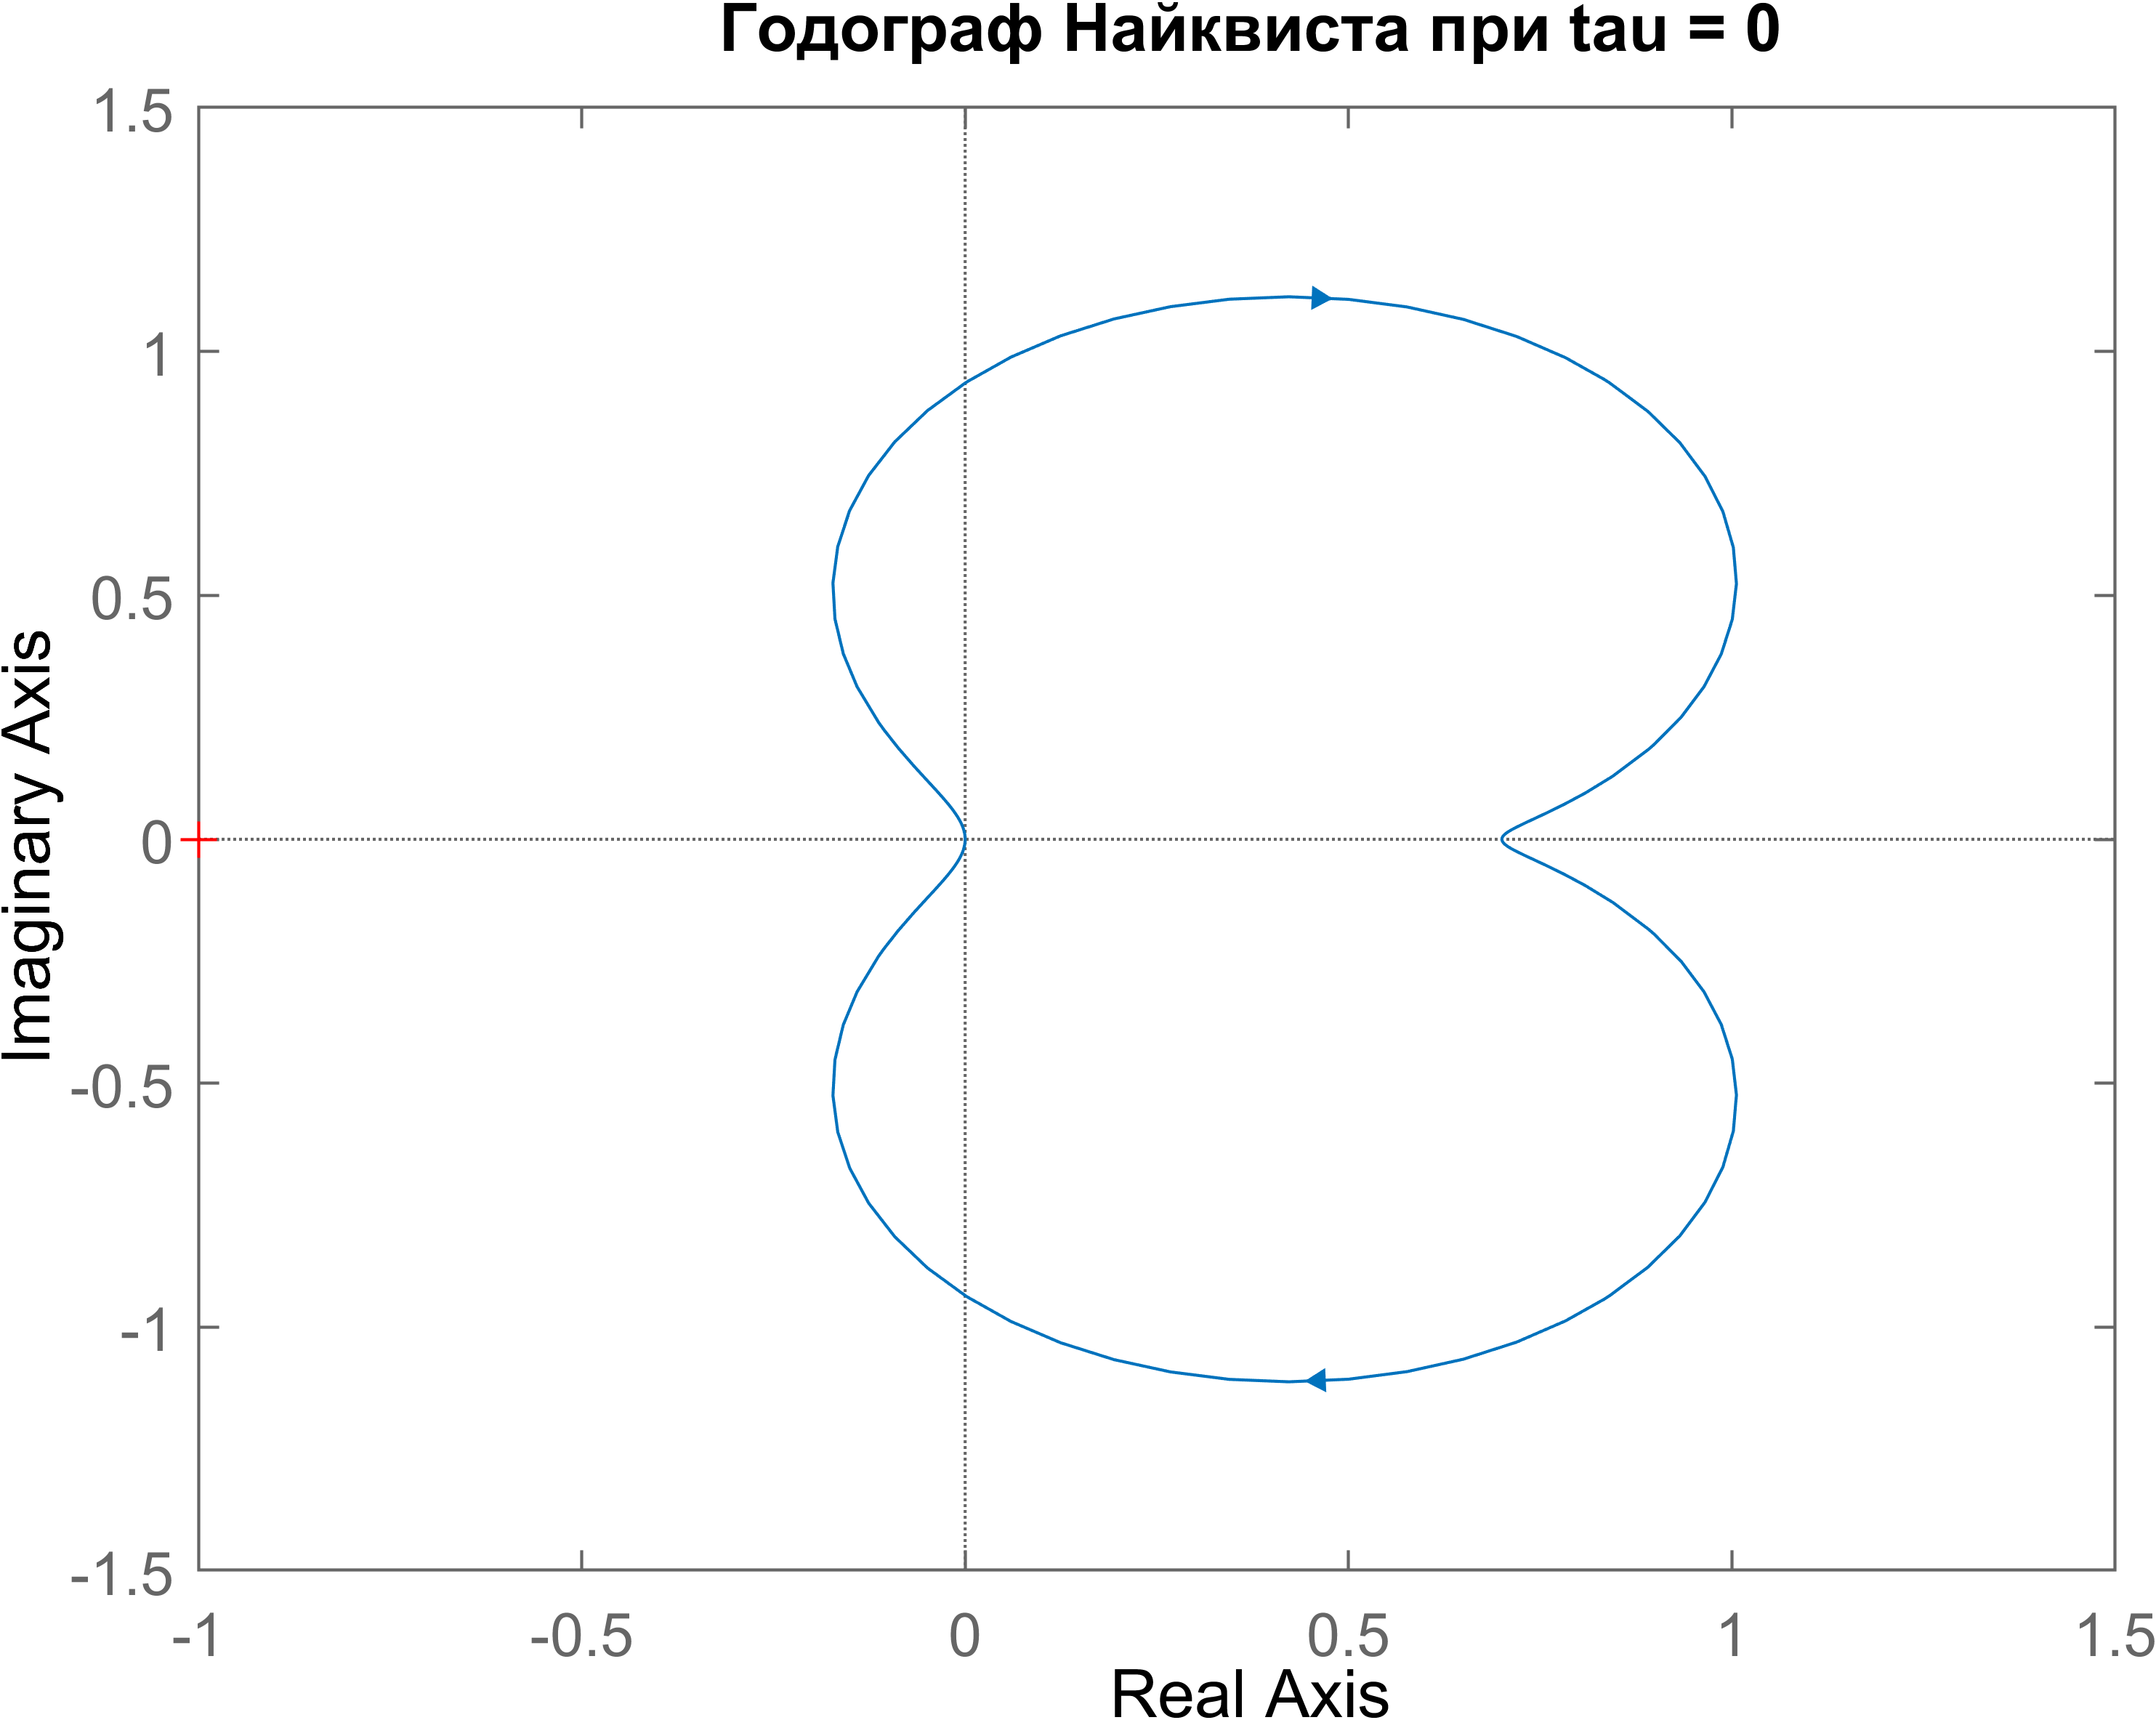
\includegraphics[width=0.7\textwidth, trim={0cm 0cm 0cm 0cm}]{../images/3_1_0_hod.png}
    \caption{Годограф Найквиста для $\tau = 0$}
\end{figure}

\begin{figure}[H]
    \centering
    \centering
    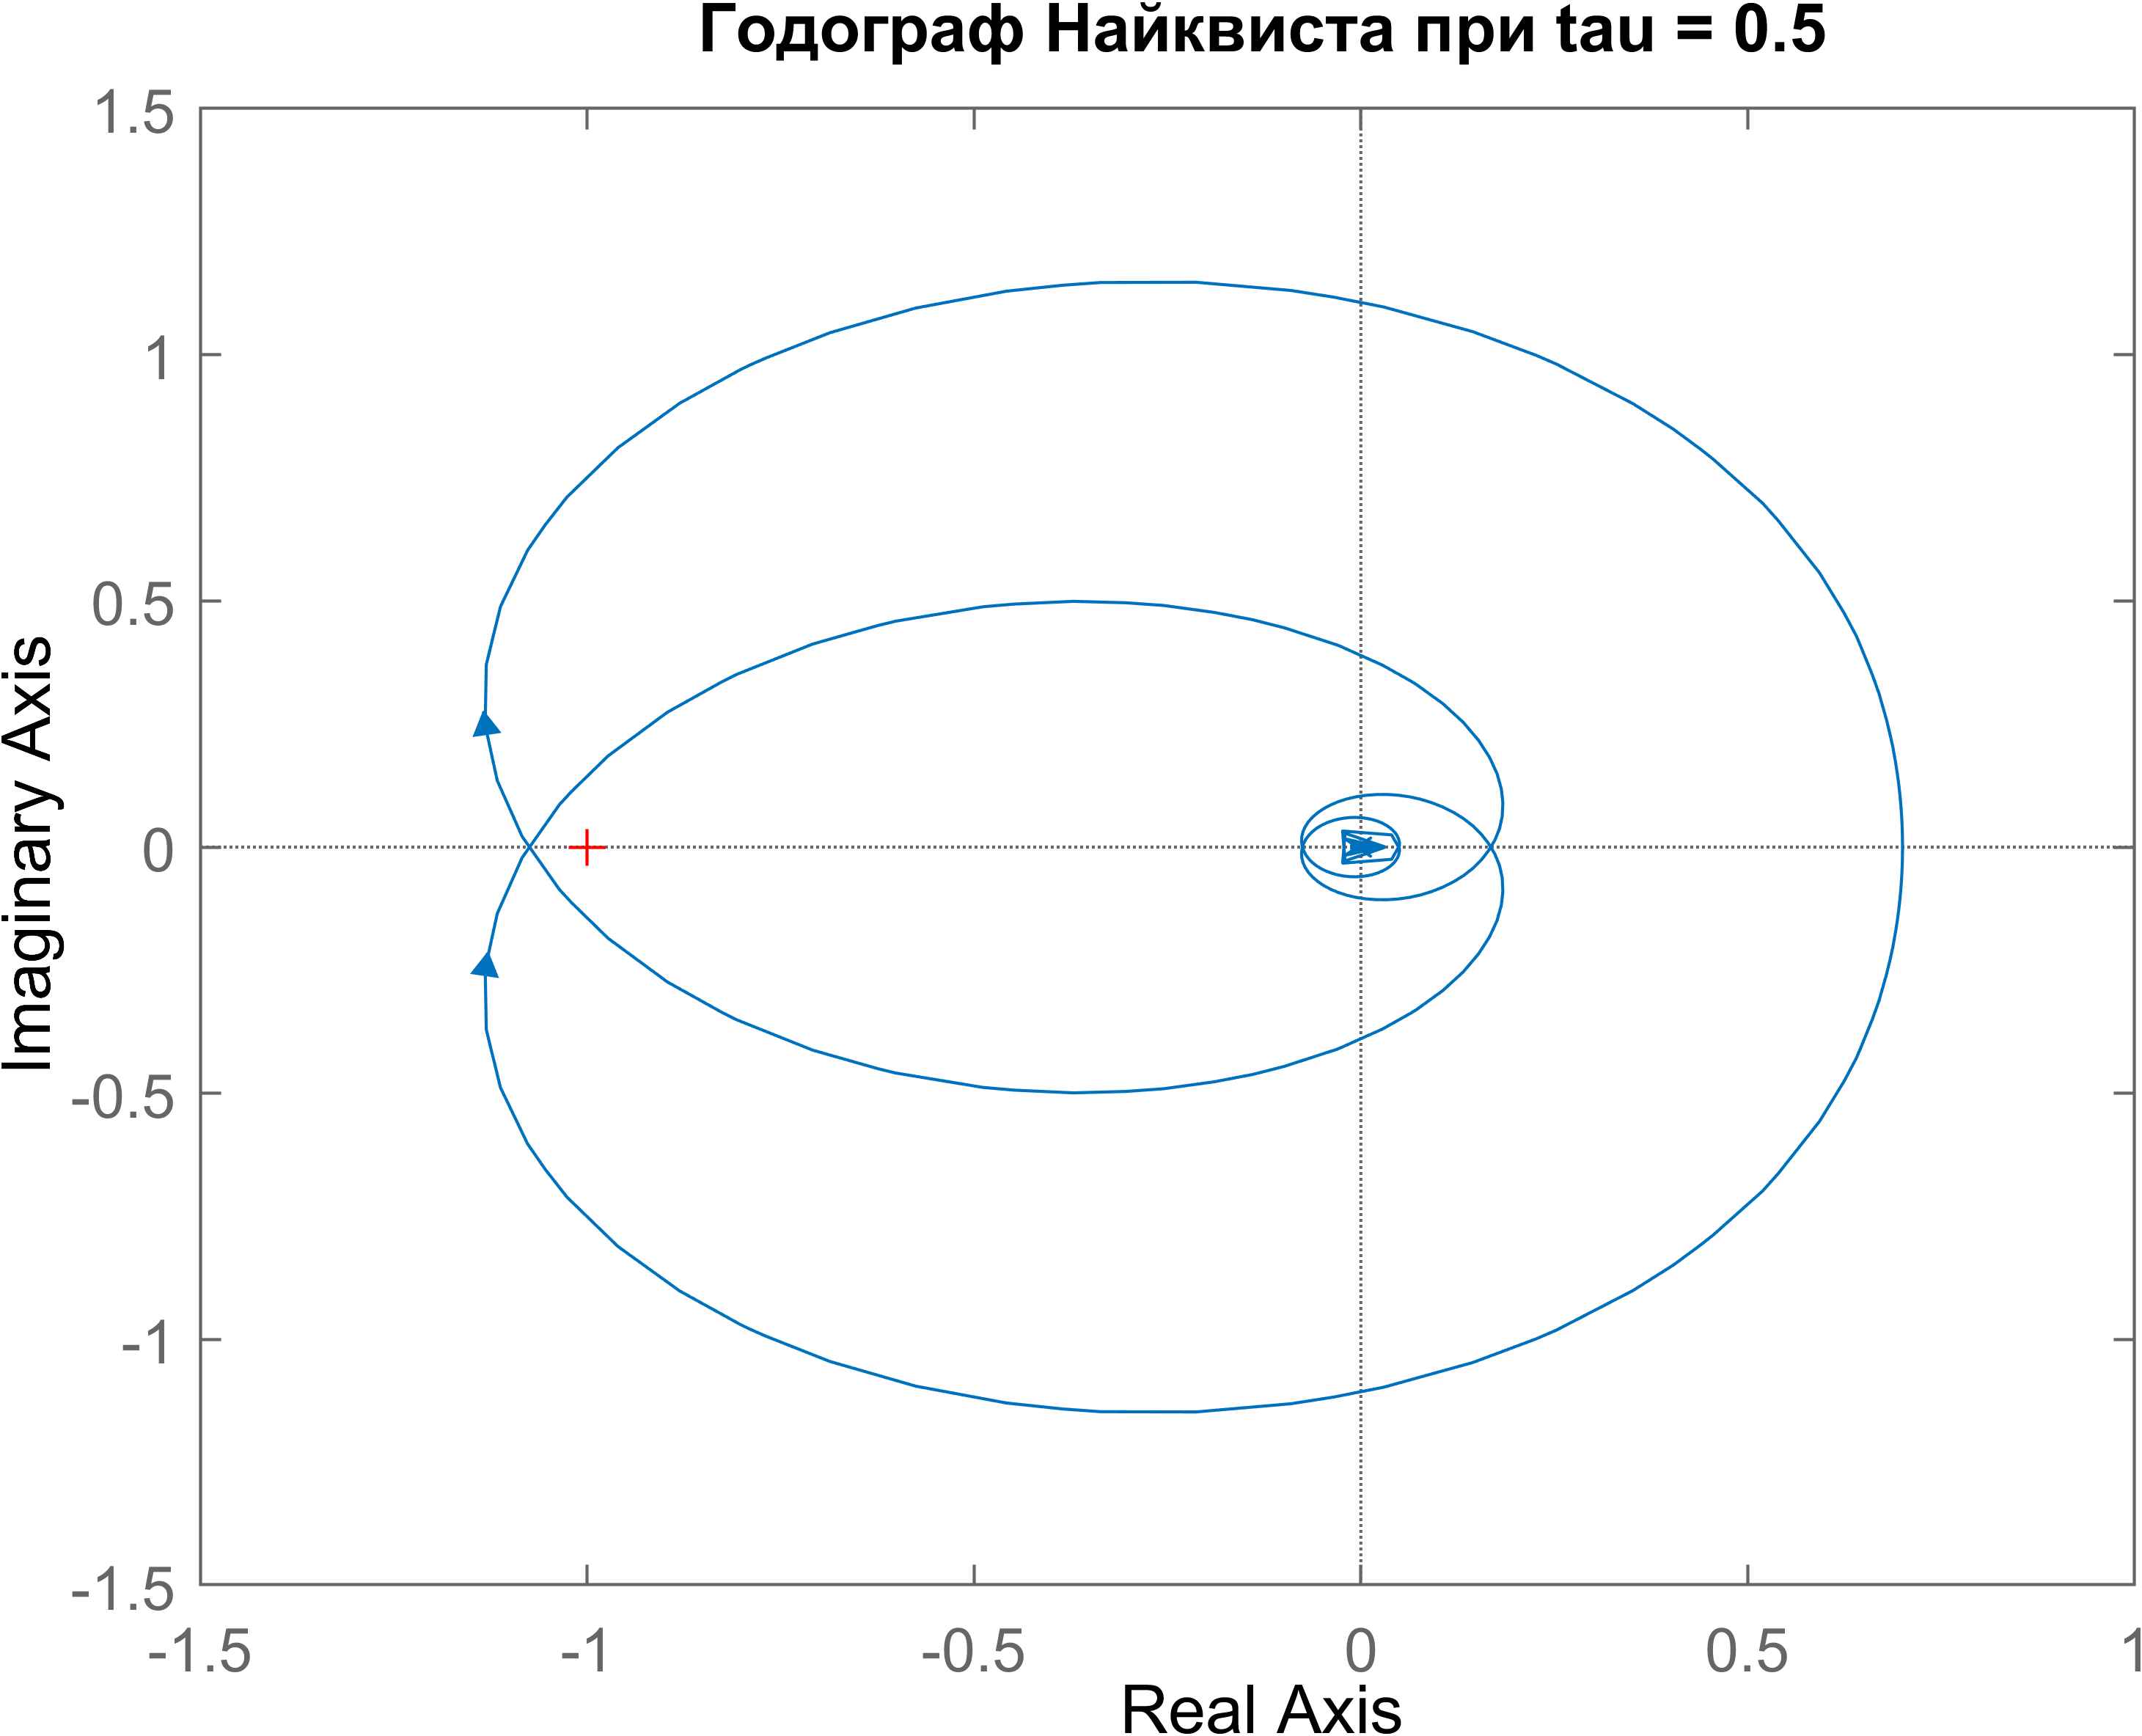
\includegraphics[width=0.7\textwidth, trim={0cm 0cm 0cm 0cm}]{../images/3_1_1_hod.png}
    \caption{Годограф Найквиста для $\tau = 0.5$}
\end{figure}

\begin{figure}[H]
    \centering
    \centering
    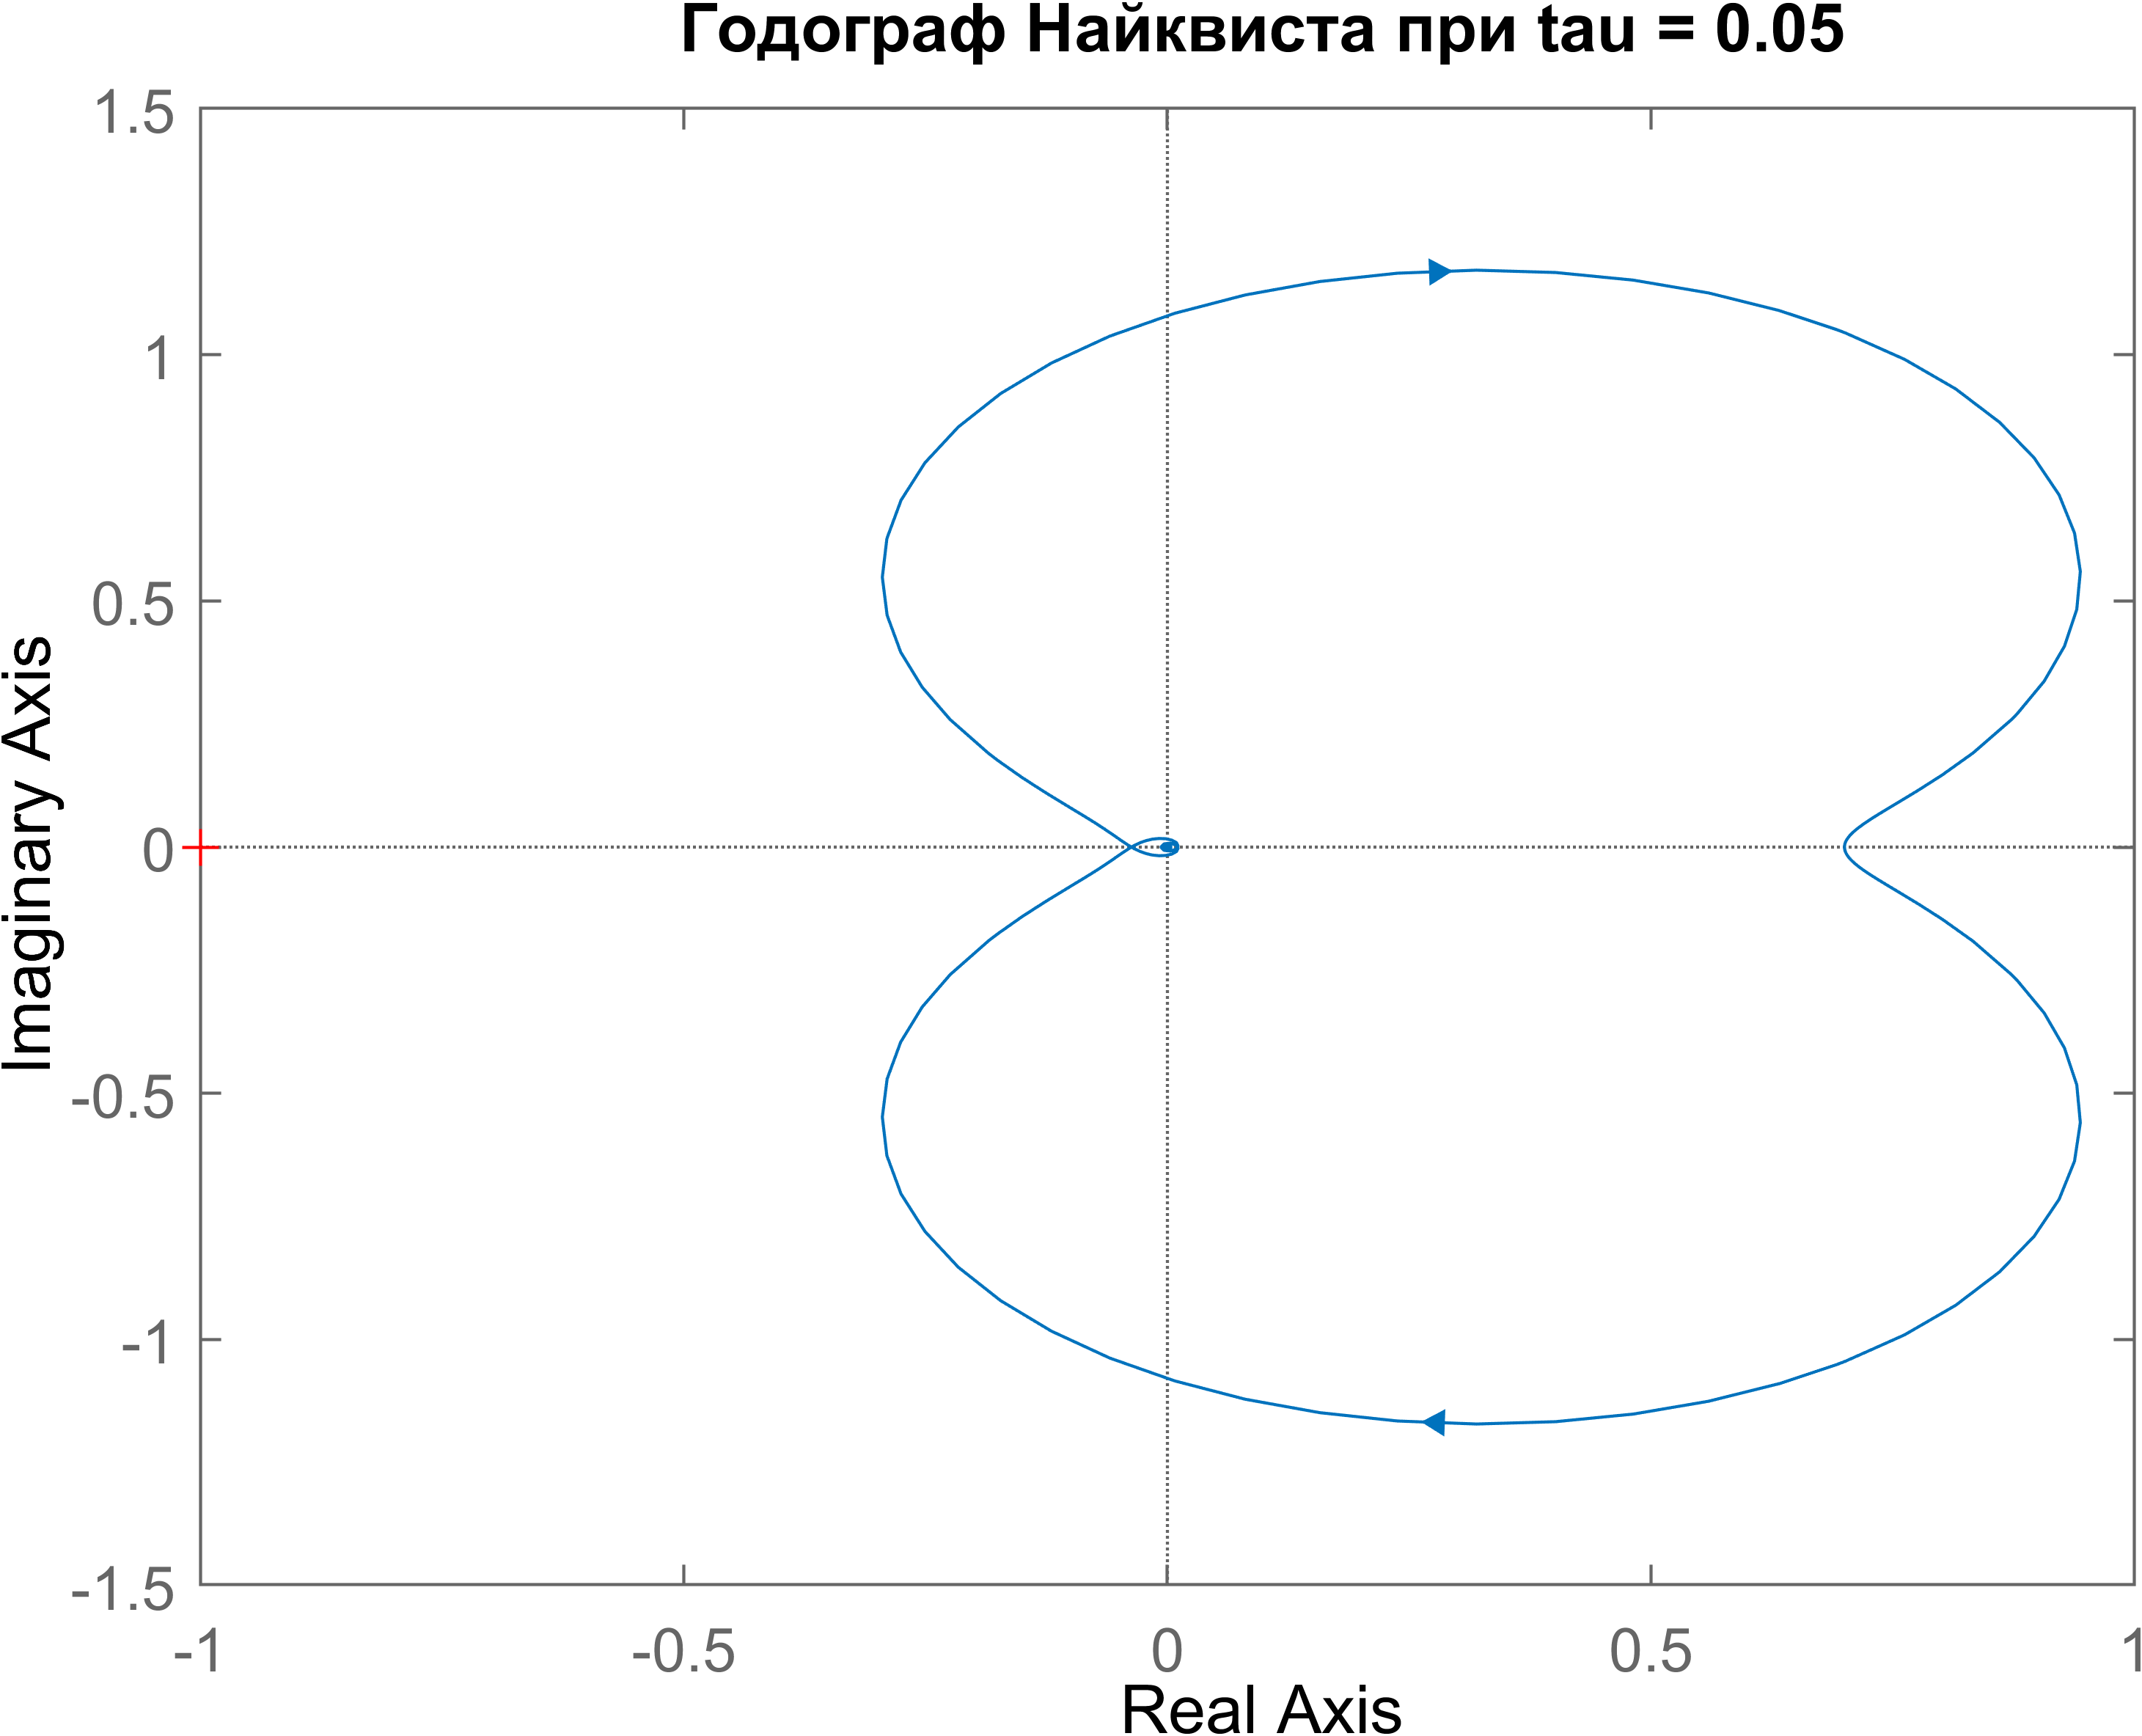
\includegraphics[width=0.7\textwidth, trim={0cm 0cm 0cm 0cm}]{../images/3_1_2_hod.png}
    \caption{Годограф Найквиста для $\tau = 0.05$}
\end{figure}

\begin{figure}[H]
    \centering
    \centering
    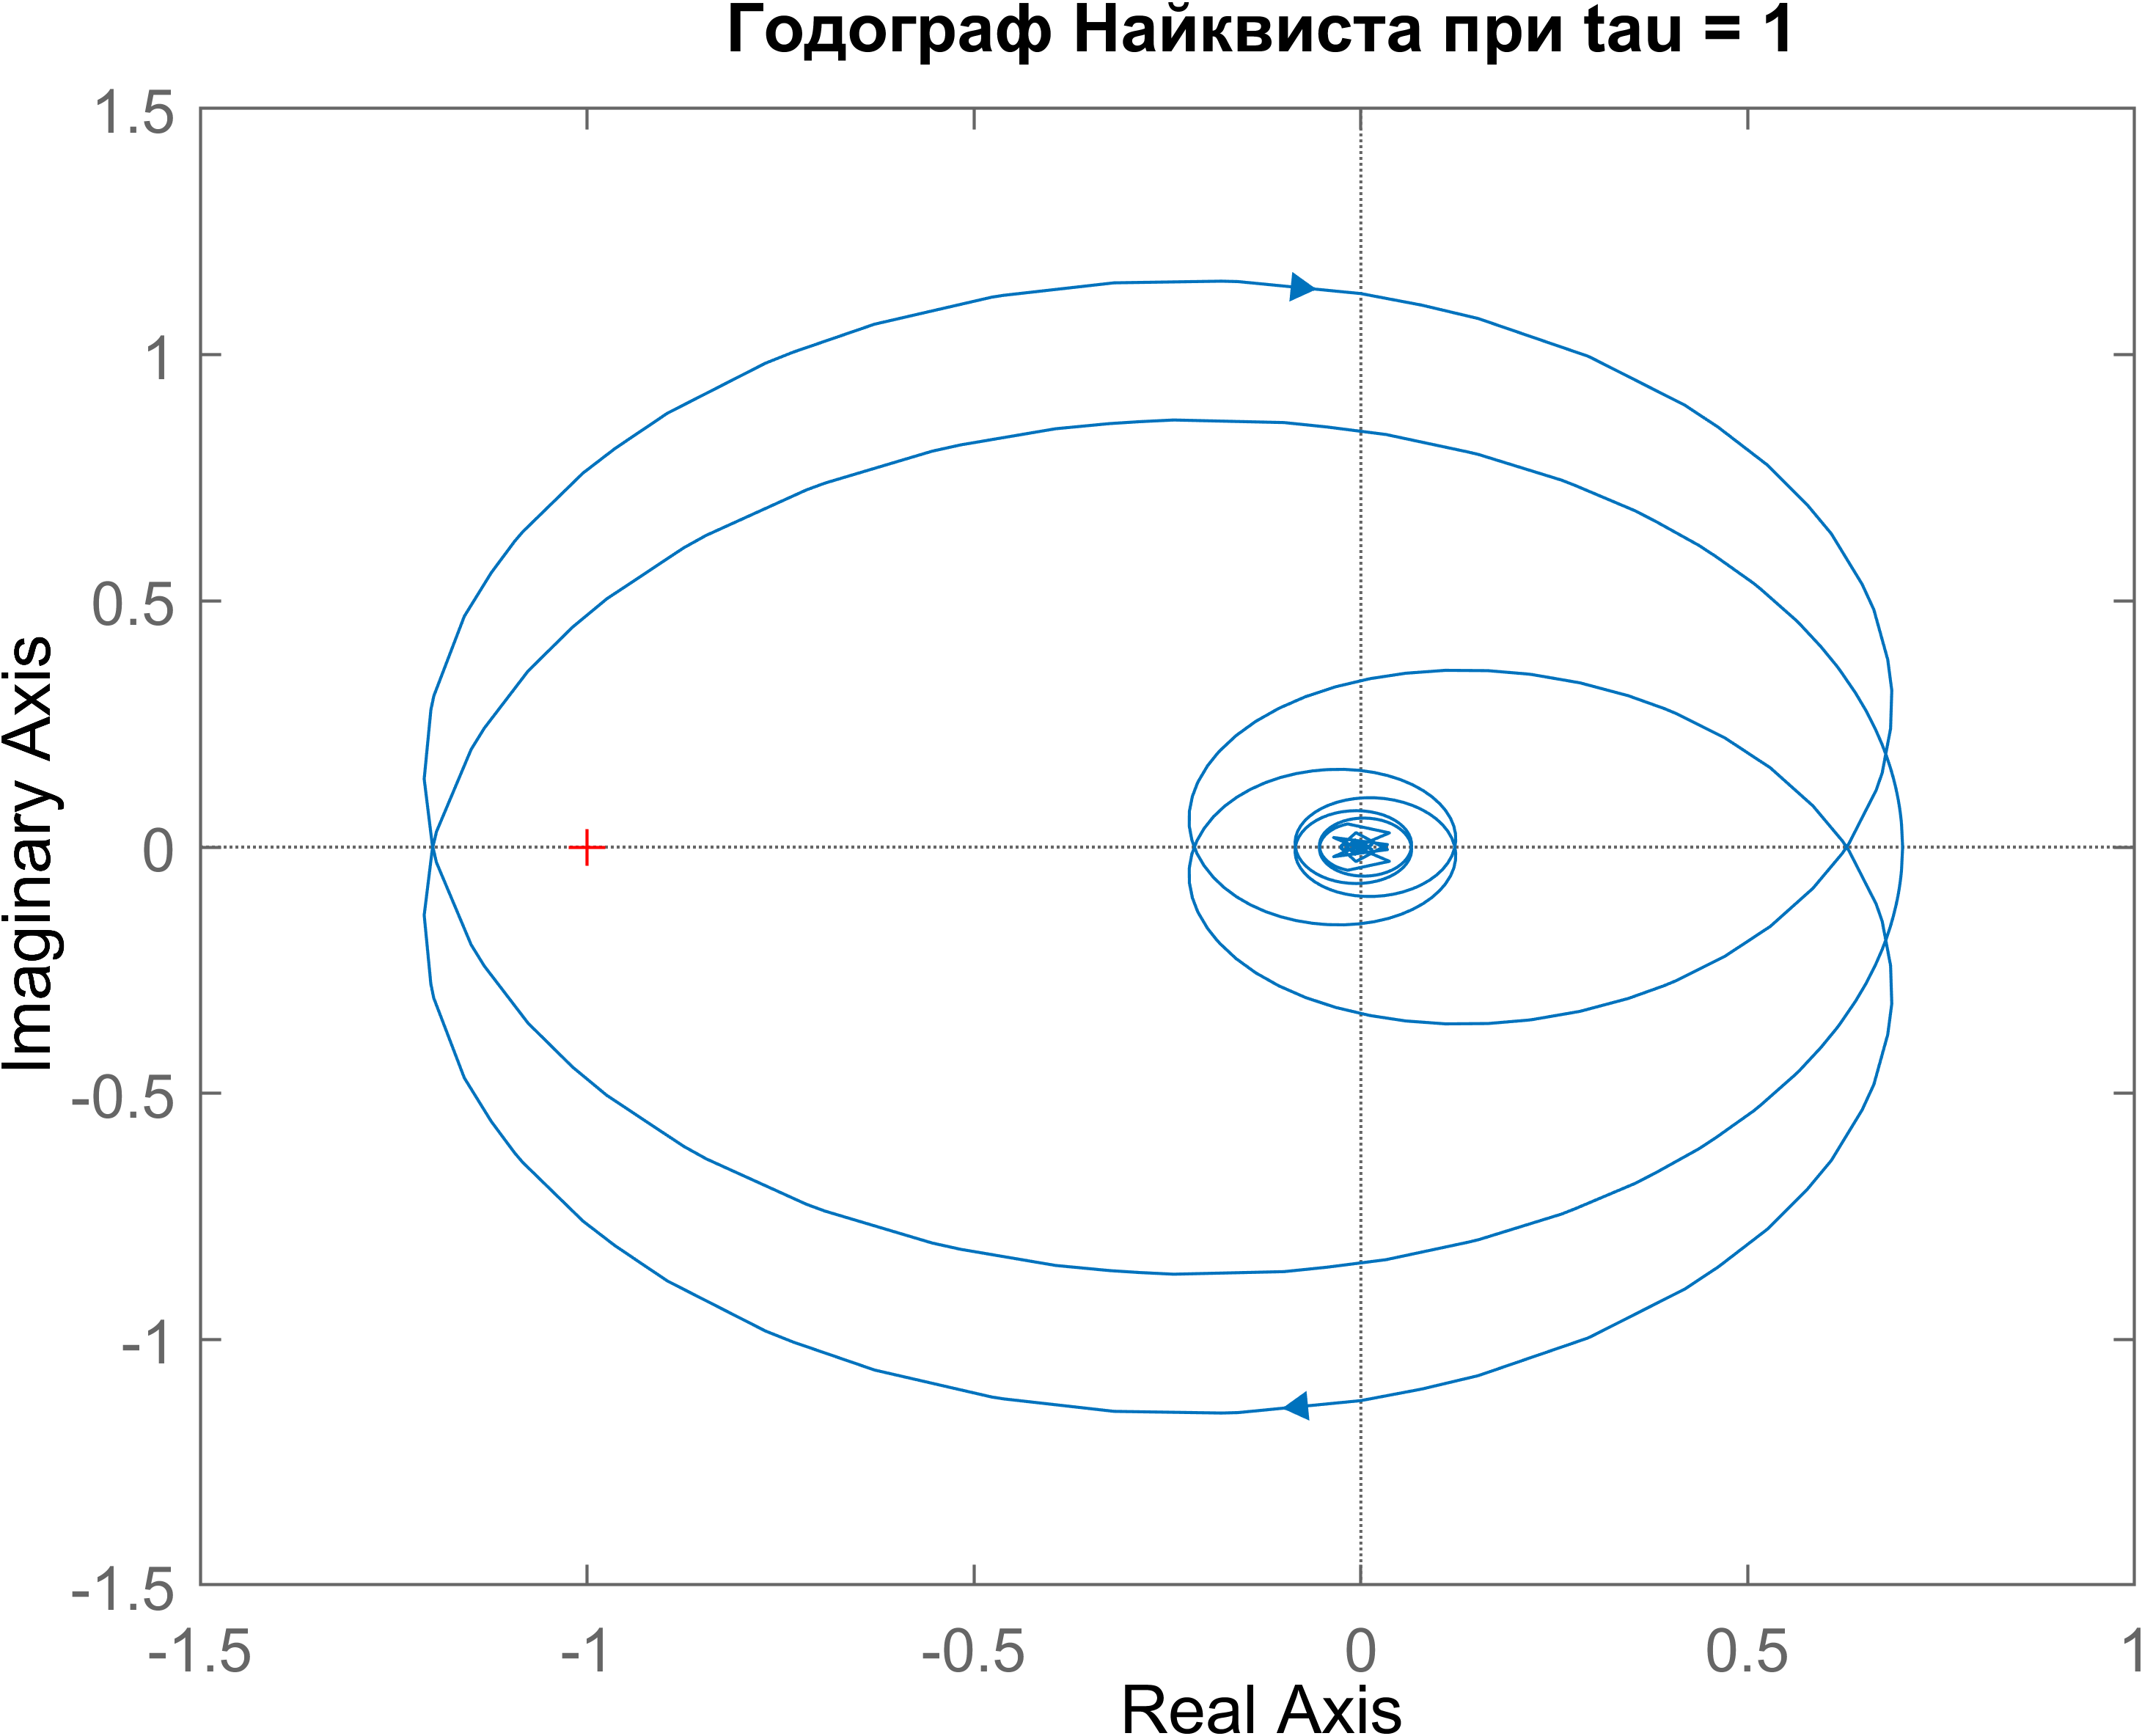
\includegraphics[width=0.7\textwidth, trim={0cm 0cm 0cm 0cm}]{../images/3_1_3_hod.png}
    \caption{Годограф Найквиста для $\tau = 1$}
\end{figure}

\begin{figure}[H]
    \centering
    \centering
    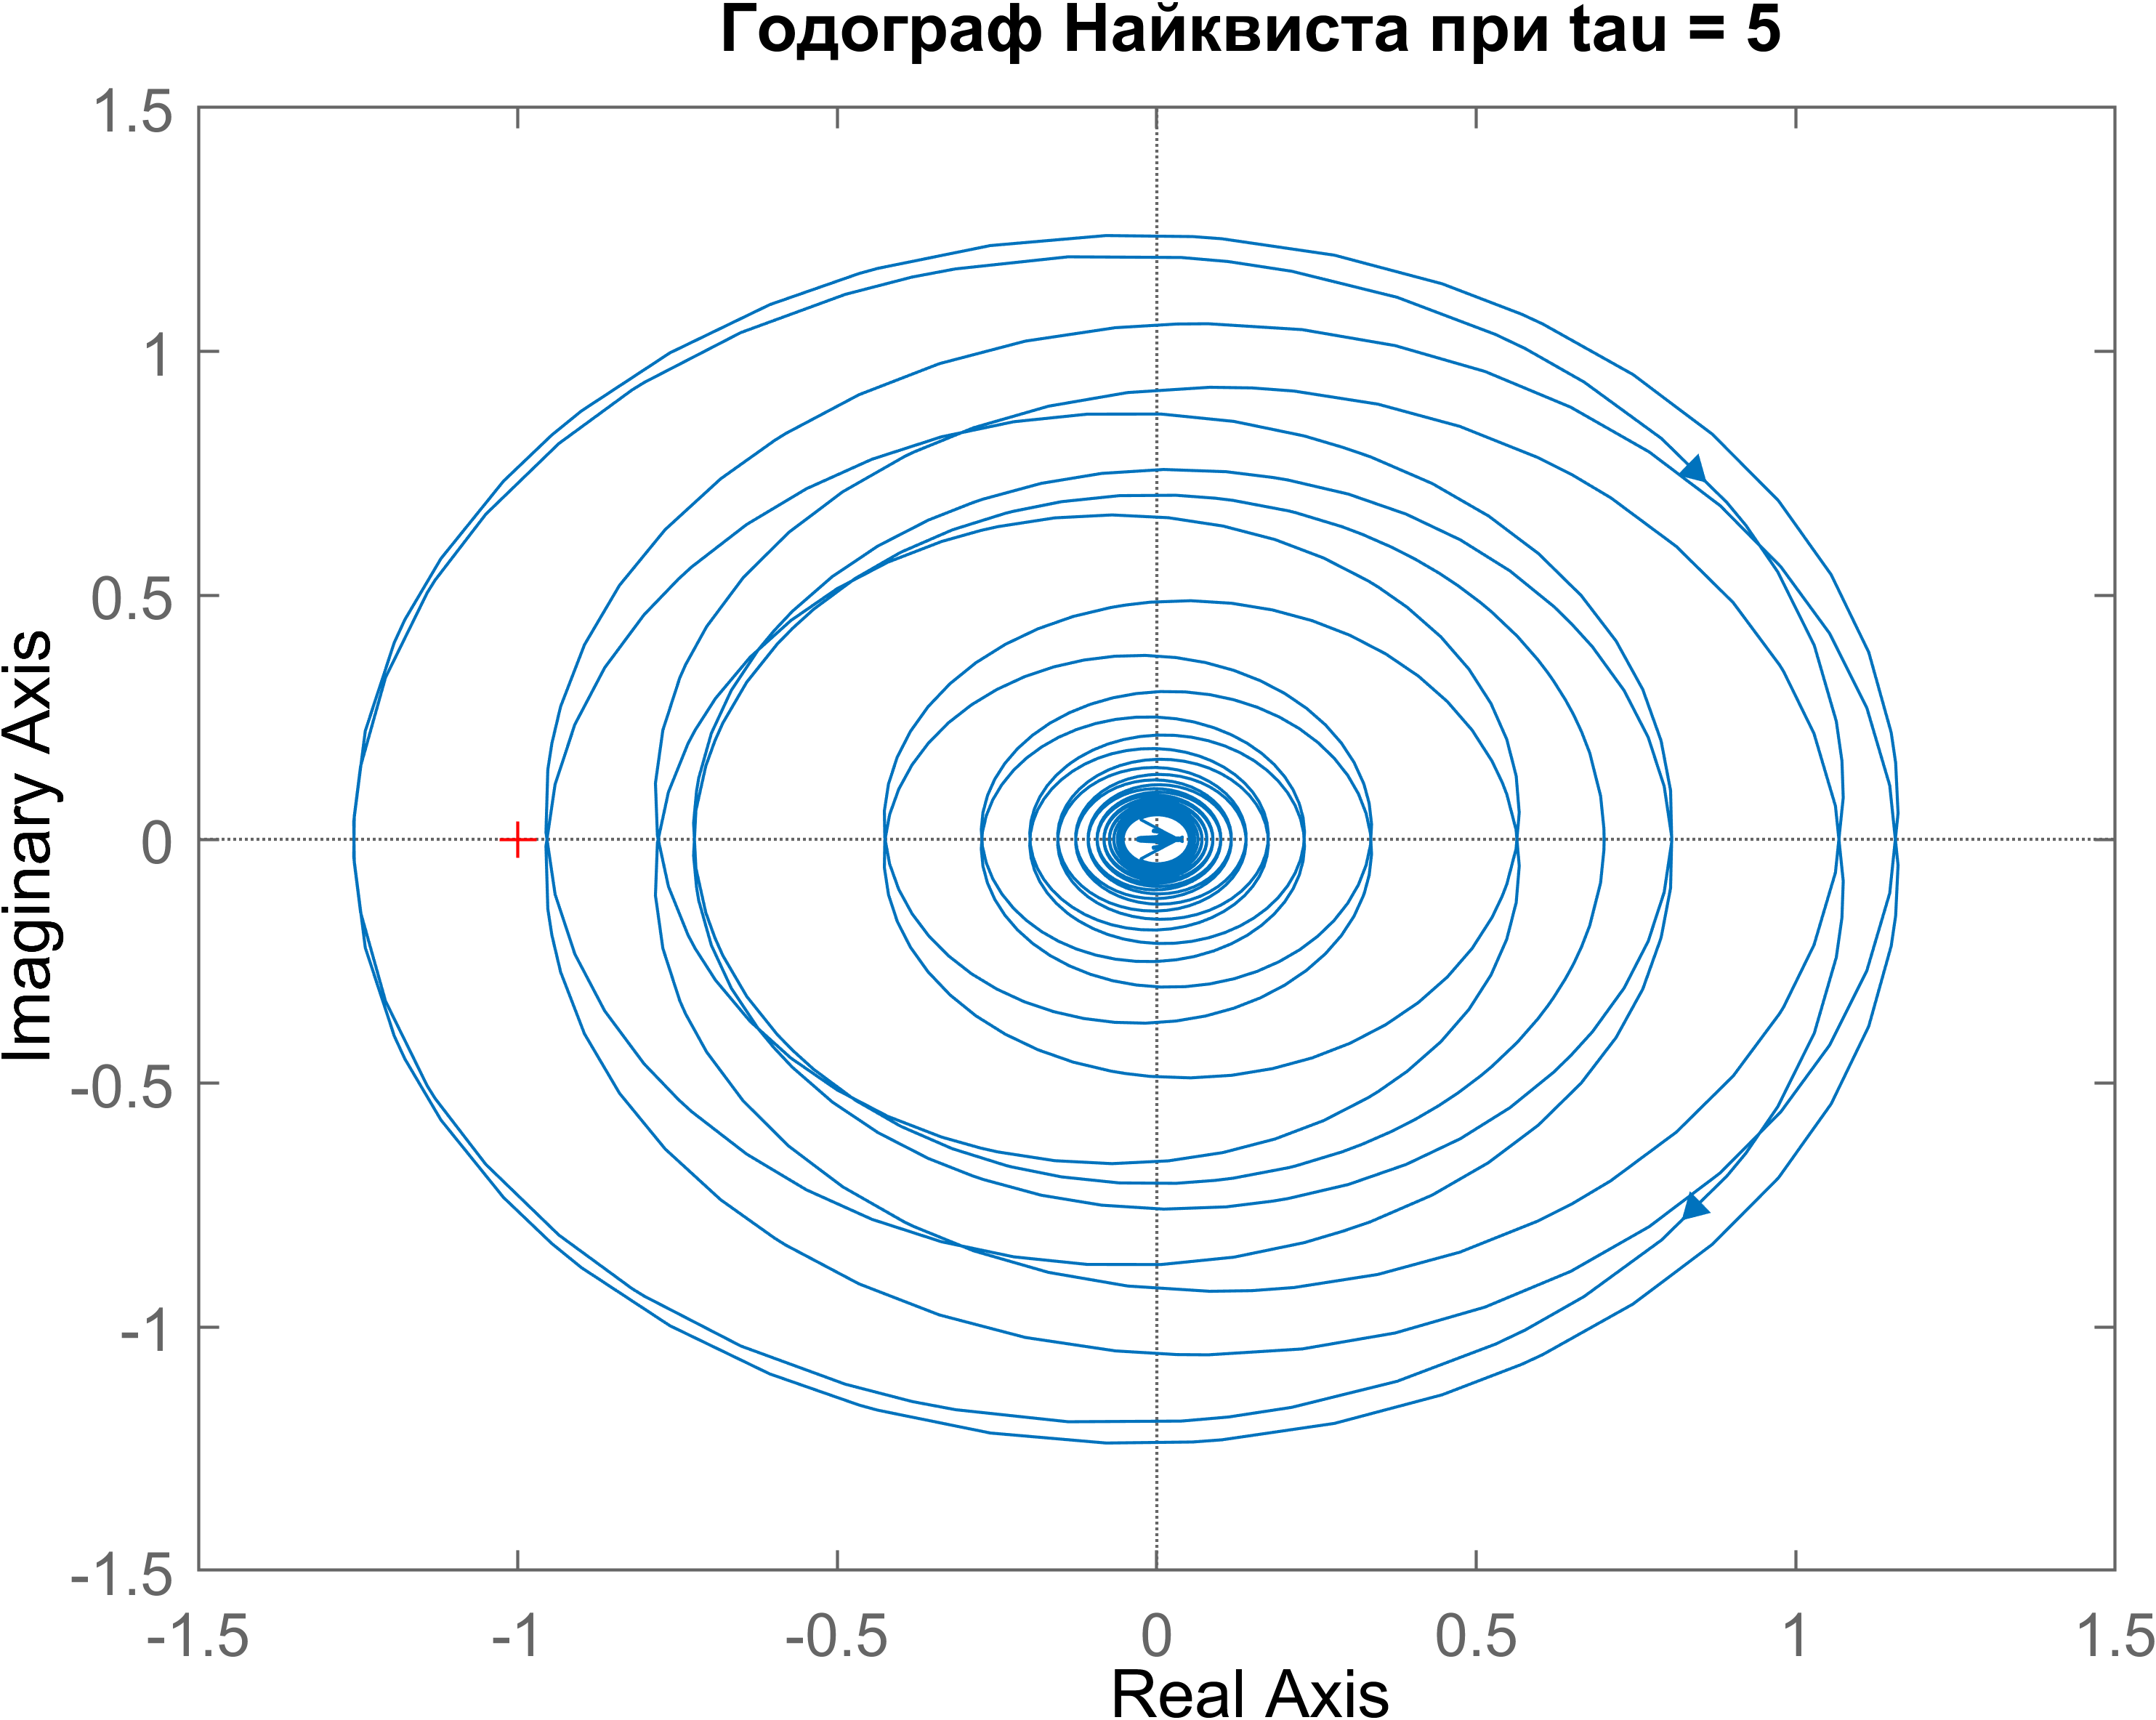
\includegraphics[width=0.7\textwidth, trim={0cm 0cm 0cm 0cm}]{../images/3_1_4_hod.png}
    \caption{Годограф Найквиста для $\tau = 5$}
\end{figure}

Как видим при увеличении запаздывания $\tau$ годограф все больше закручивается. Для 
того чтобы найти граничные значения при которых система остается устойчивой, найдем
сначала частотные характеристики системы:
\[
W_3(j\omega) = \frac{-5w^2 - 70 + (-w^3 + 4w)j}{w^4 - 16w^2 + 100}
\]
\[
A(w) = \frac{\sqrt{w^2 + 49}}{\sqrt{w^4 - 16w^2 + 100}}
\]
\[
\varphi(w) = \text{atan2}\left(\frac{-w^3 + 4w}{w^4 - 16w^2 + 100}, \frac{-5w^2 - 70}{w^4 - 16w^2 + 100}\right)
\]

Частоты среза имеют значения:
\[
w_{cp1} = 1.97, \quad w_{cp2} = 3.62
\]

Запас по фазе:
\[
\varphi_{p1} = \pi + \varphi(w_{cp1}) = \pi - 0.3 = 2.84
\]
\[
\tau_1 = \frac{\varphi_{p1}}{w_{cp1}} = 1.44
\]
\[
\varphi_{p2} = \pi + \varphi(w_{cp2}) = \pi - 1.5 = 1.64
\]

\[
\tau_2 = \frac{\varphi_{p2}}{w_{cp2}} = 0.45
\]

Таким образом, система остается устойчивой при $\tau < 0.45$ и $\tau > 1.44$. Продемонстрируем переходные 
характеристики системы при коэффициентах $\tau$, соответствующих устойчивости и неустойчивости для каждой из областей:
\begin{figure}[H]
    \centering
    \begin{minipage}{0.45\textwidth}
        \centering
        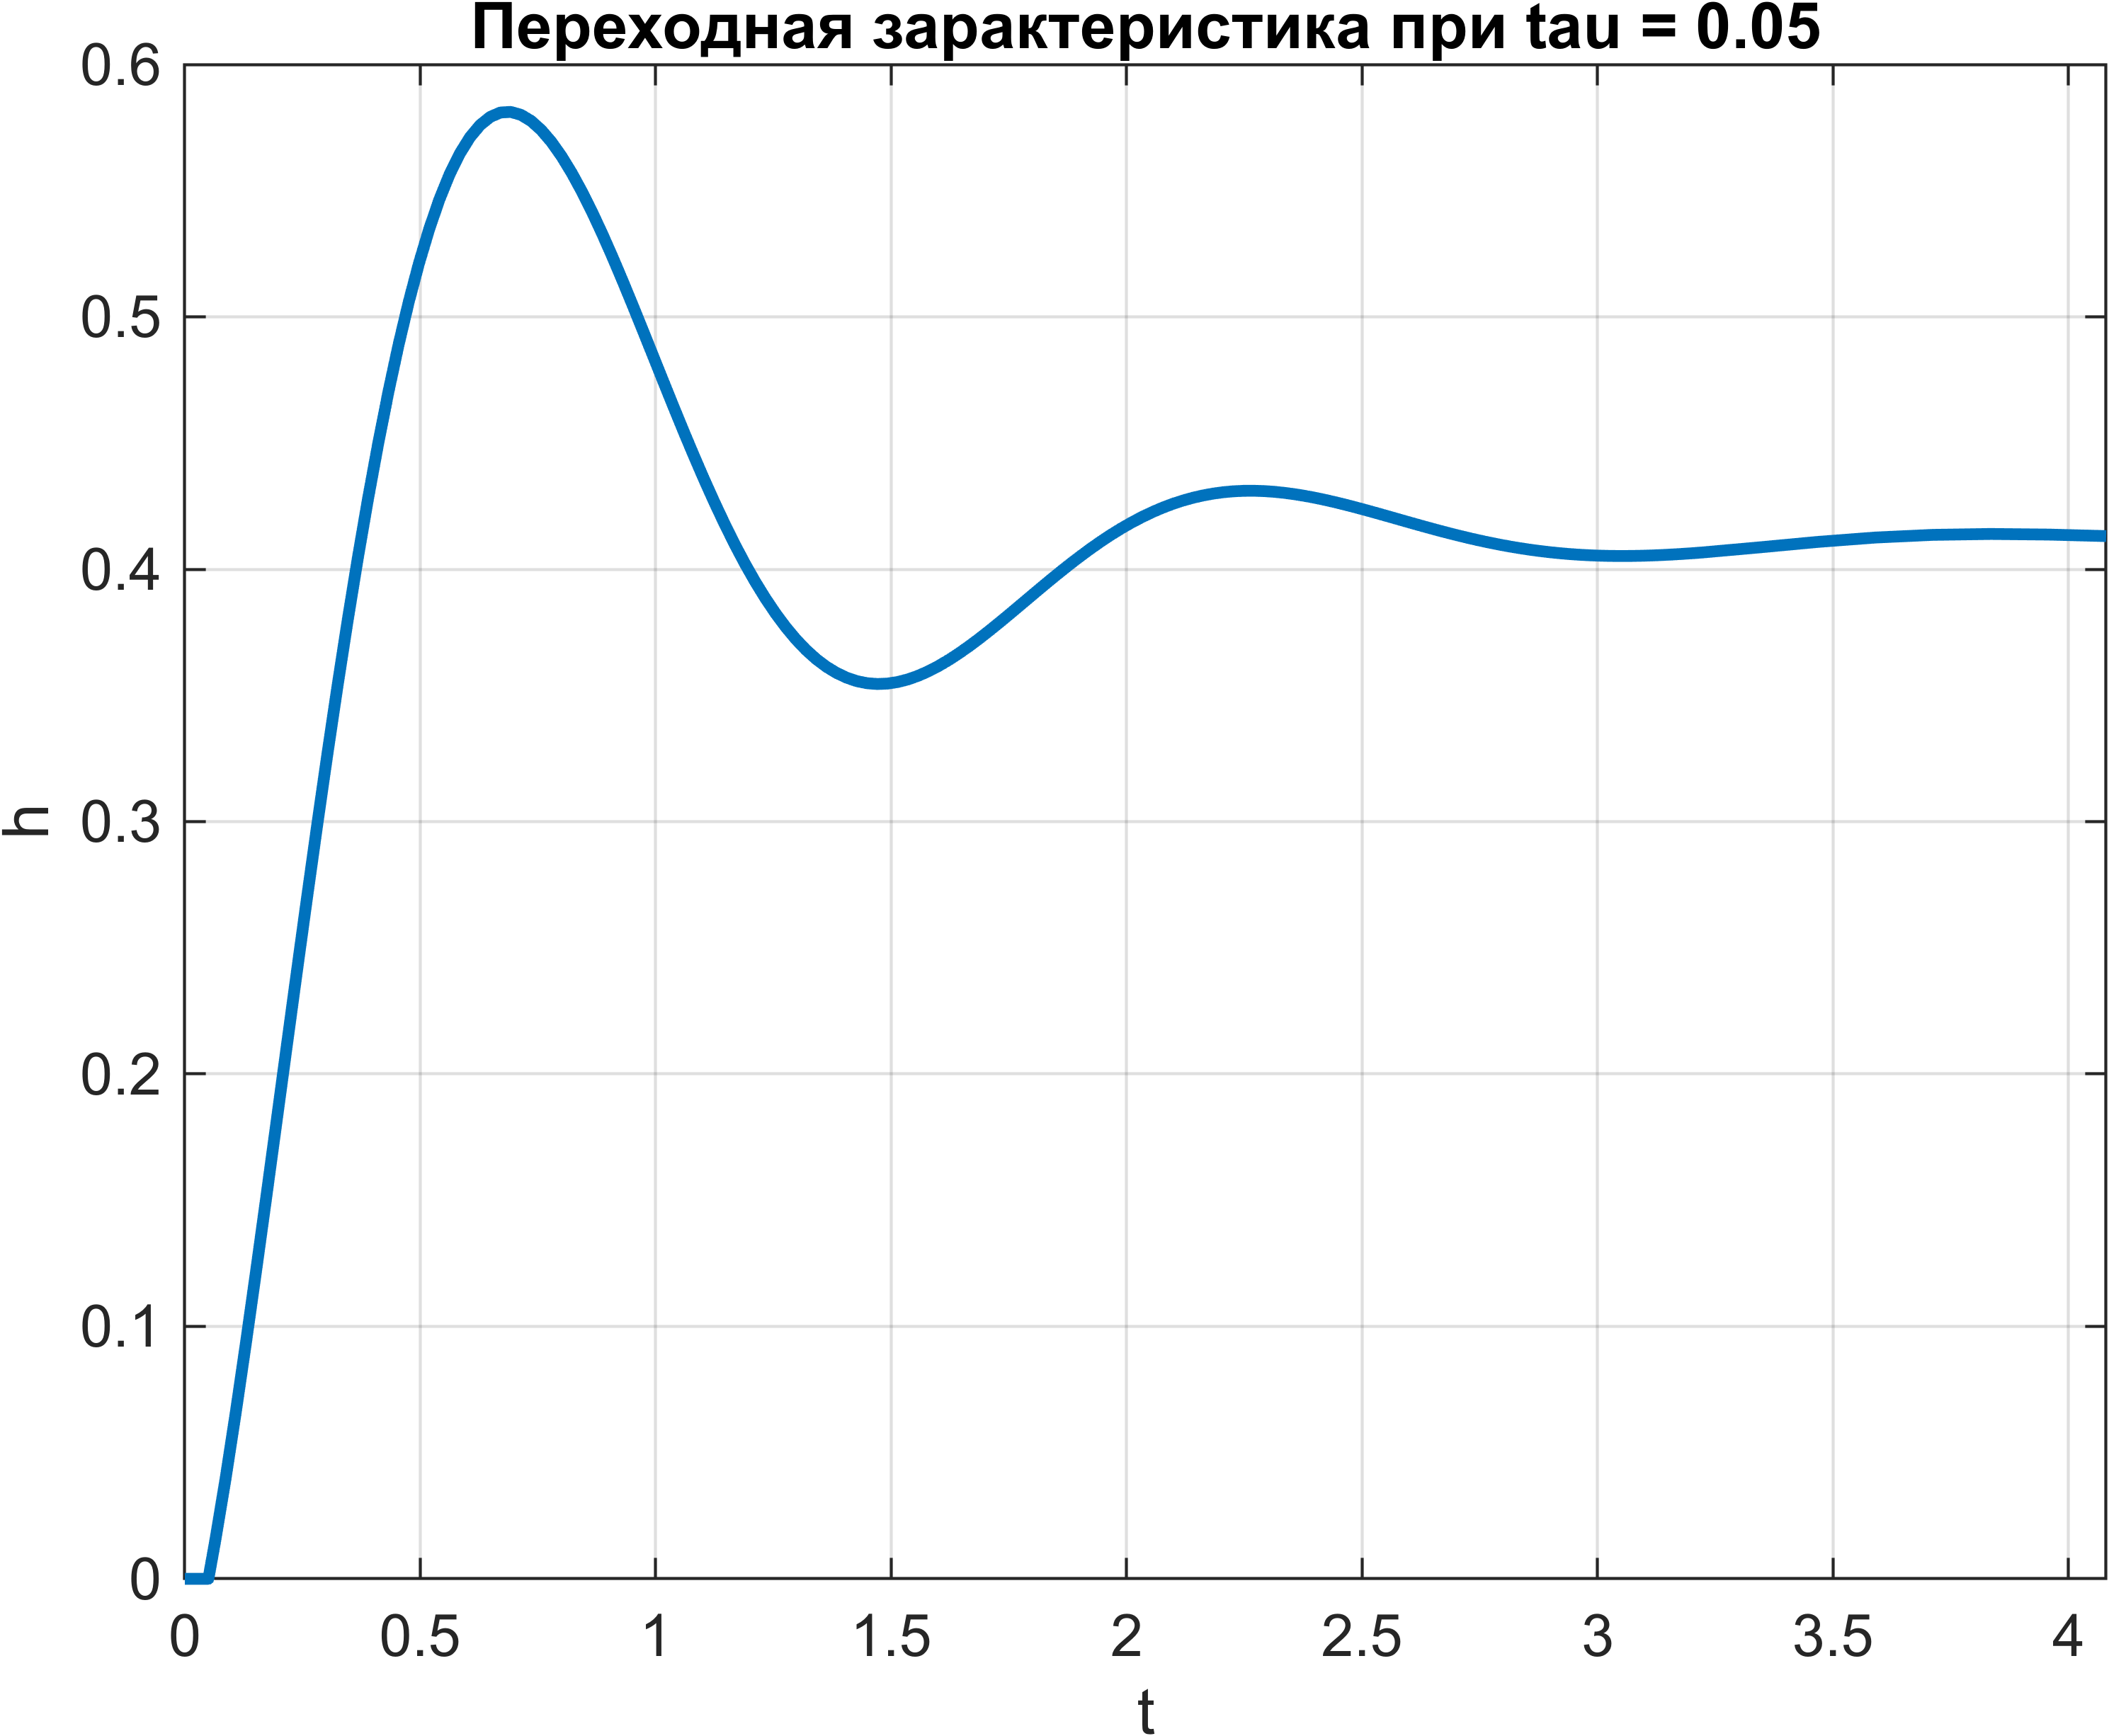
\includegraphics[width=\textwidth, trim={0cm 0cm 0cm 0cm}]{../images/3_1_5_cl.png}
    \end{minipage}
    \hfill
    \begin{minipage}{0.45\textwidth}
        \centering
        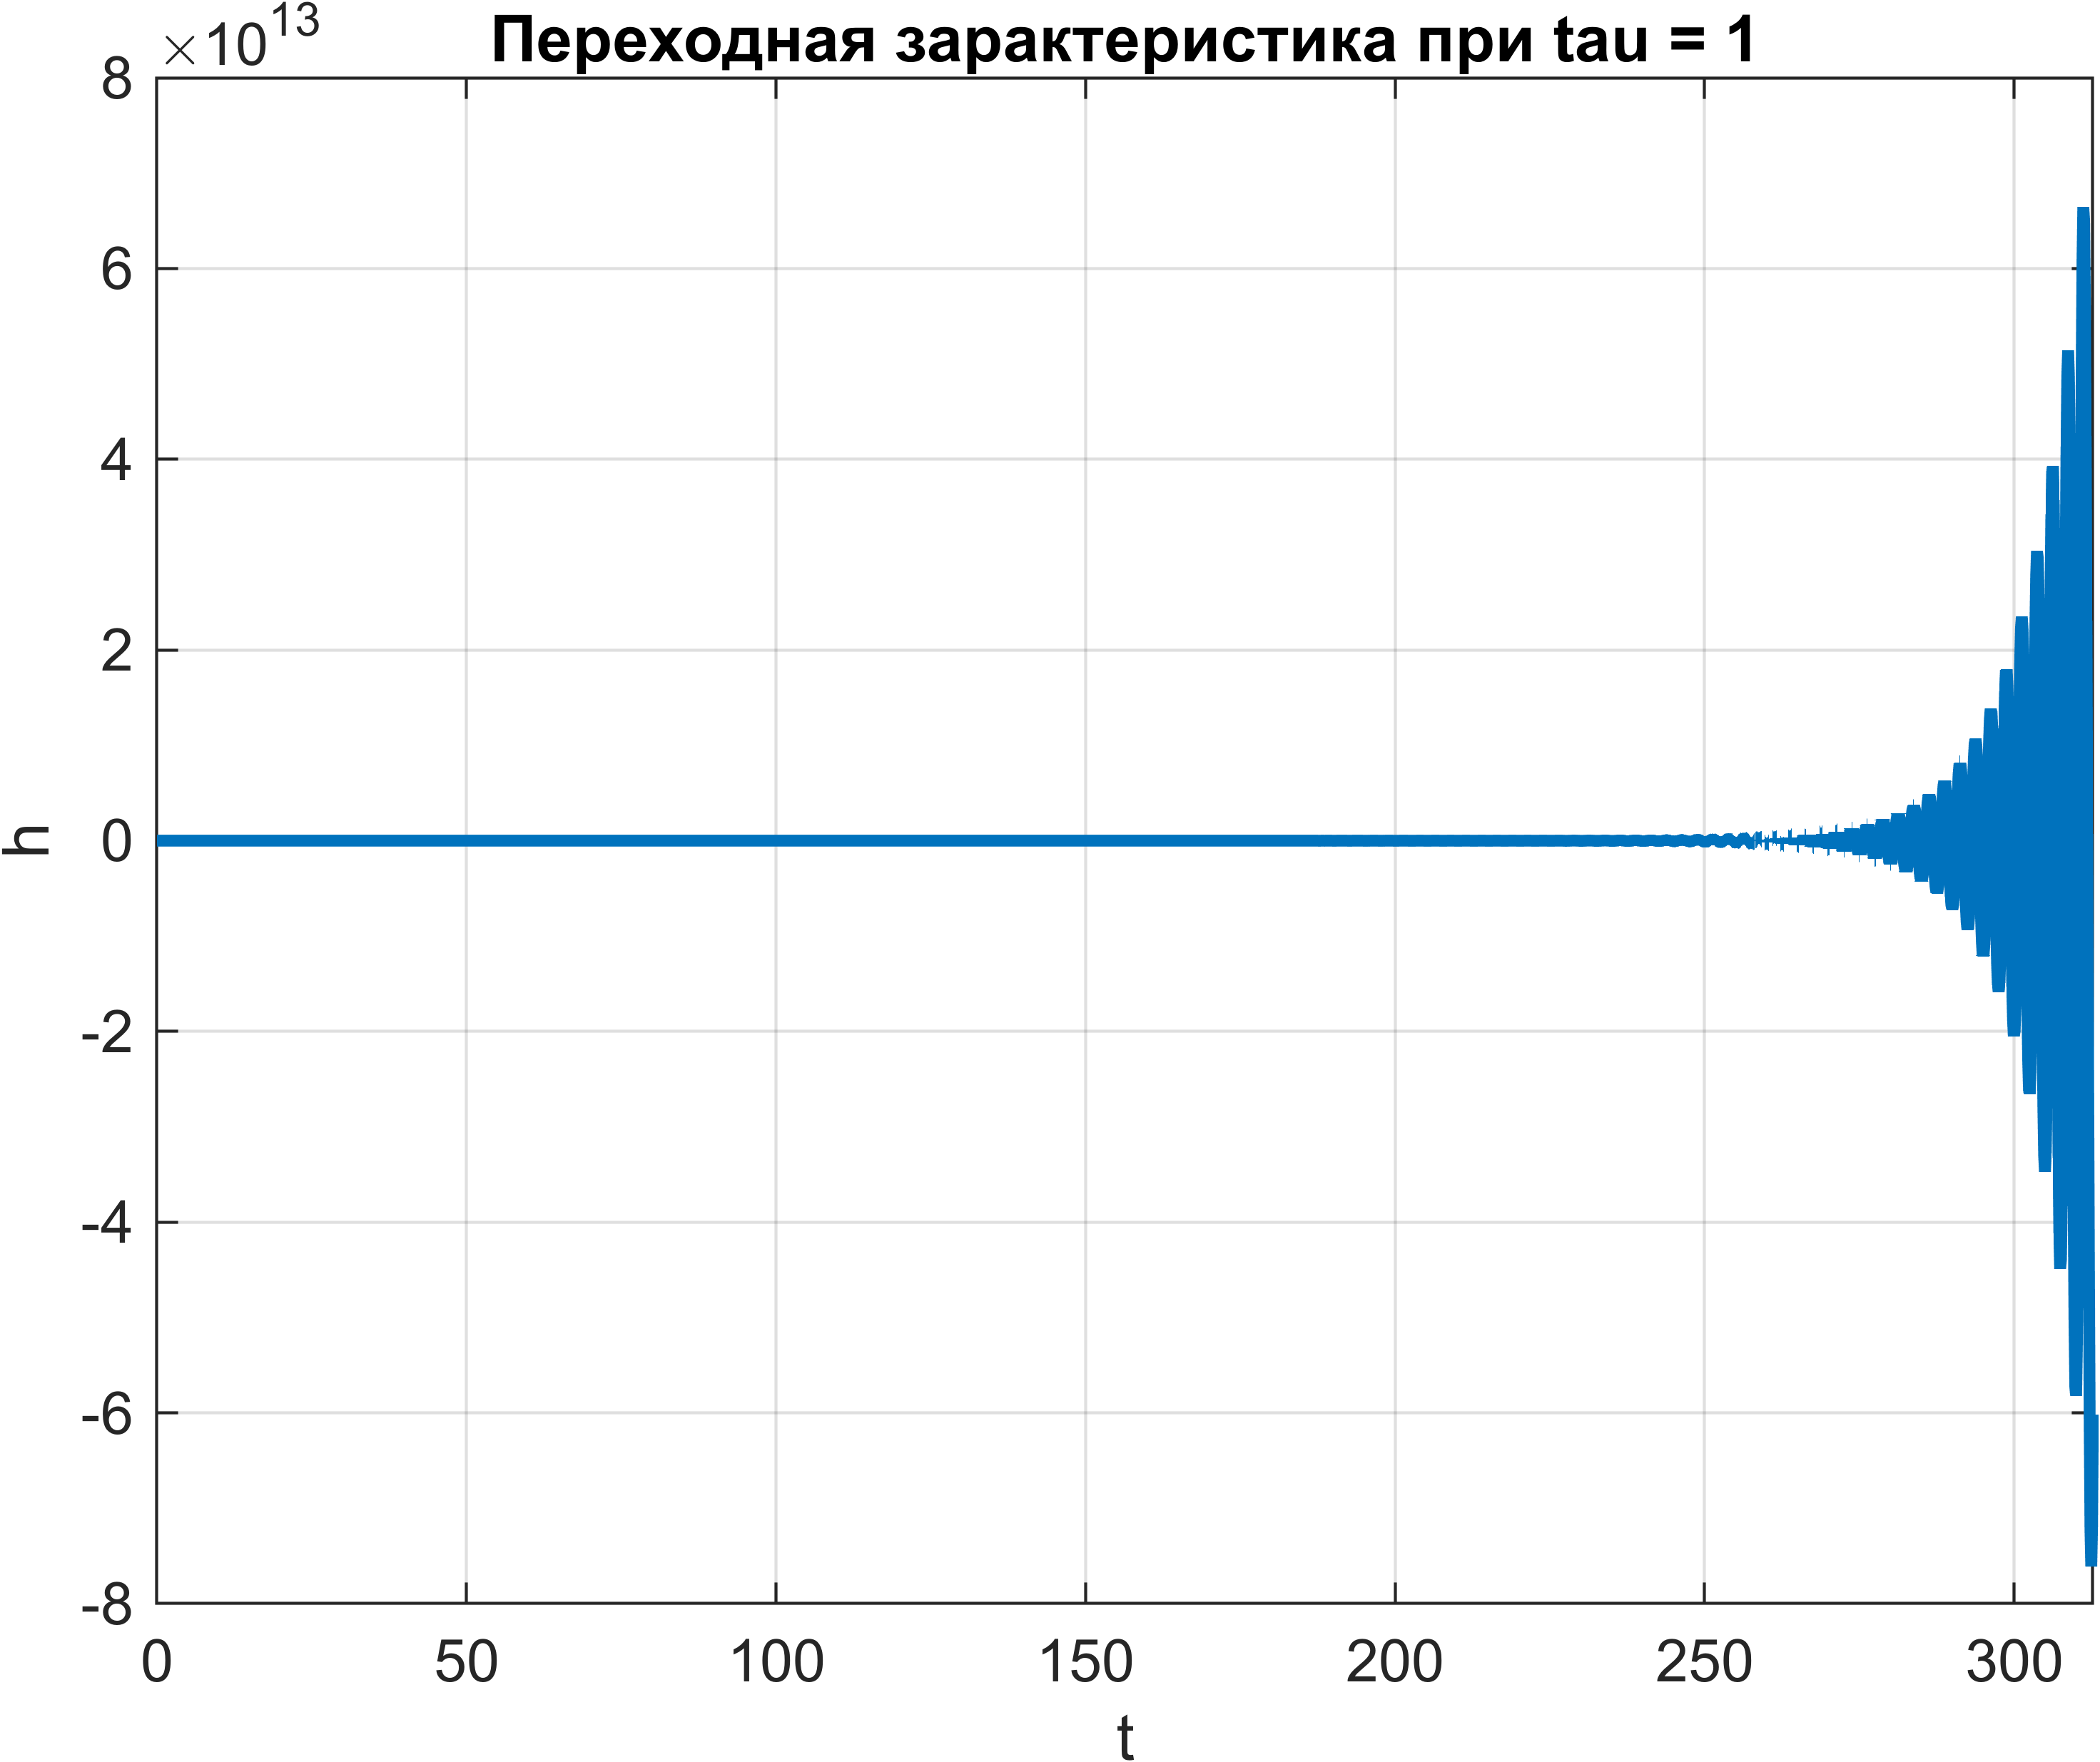
\includegraphics[width=\textwidth, trim={0cm 0cm 0cm 0cm}]{../images/3_1_6_cl.png}
    \end{minipage}
    \vfill
    \begin{minipage}{0.45\textwidth}
        \centering
        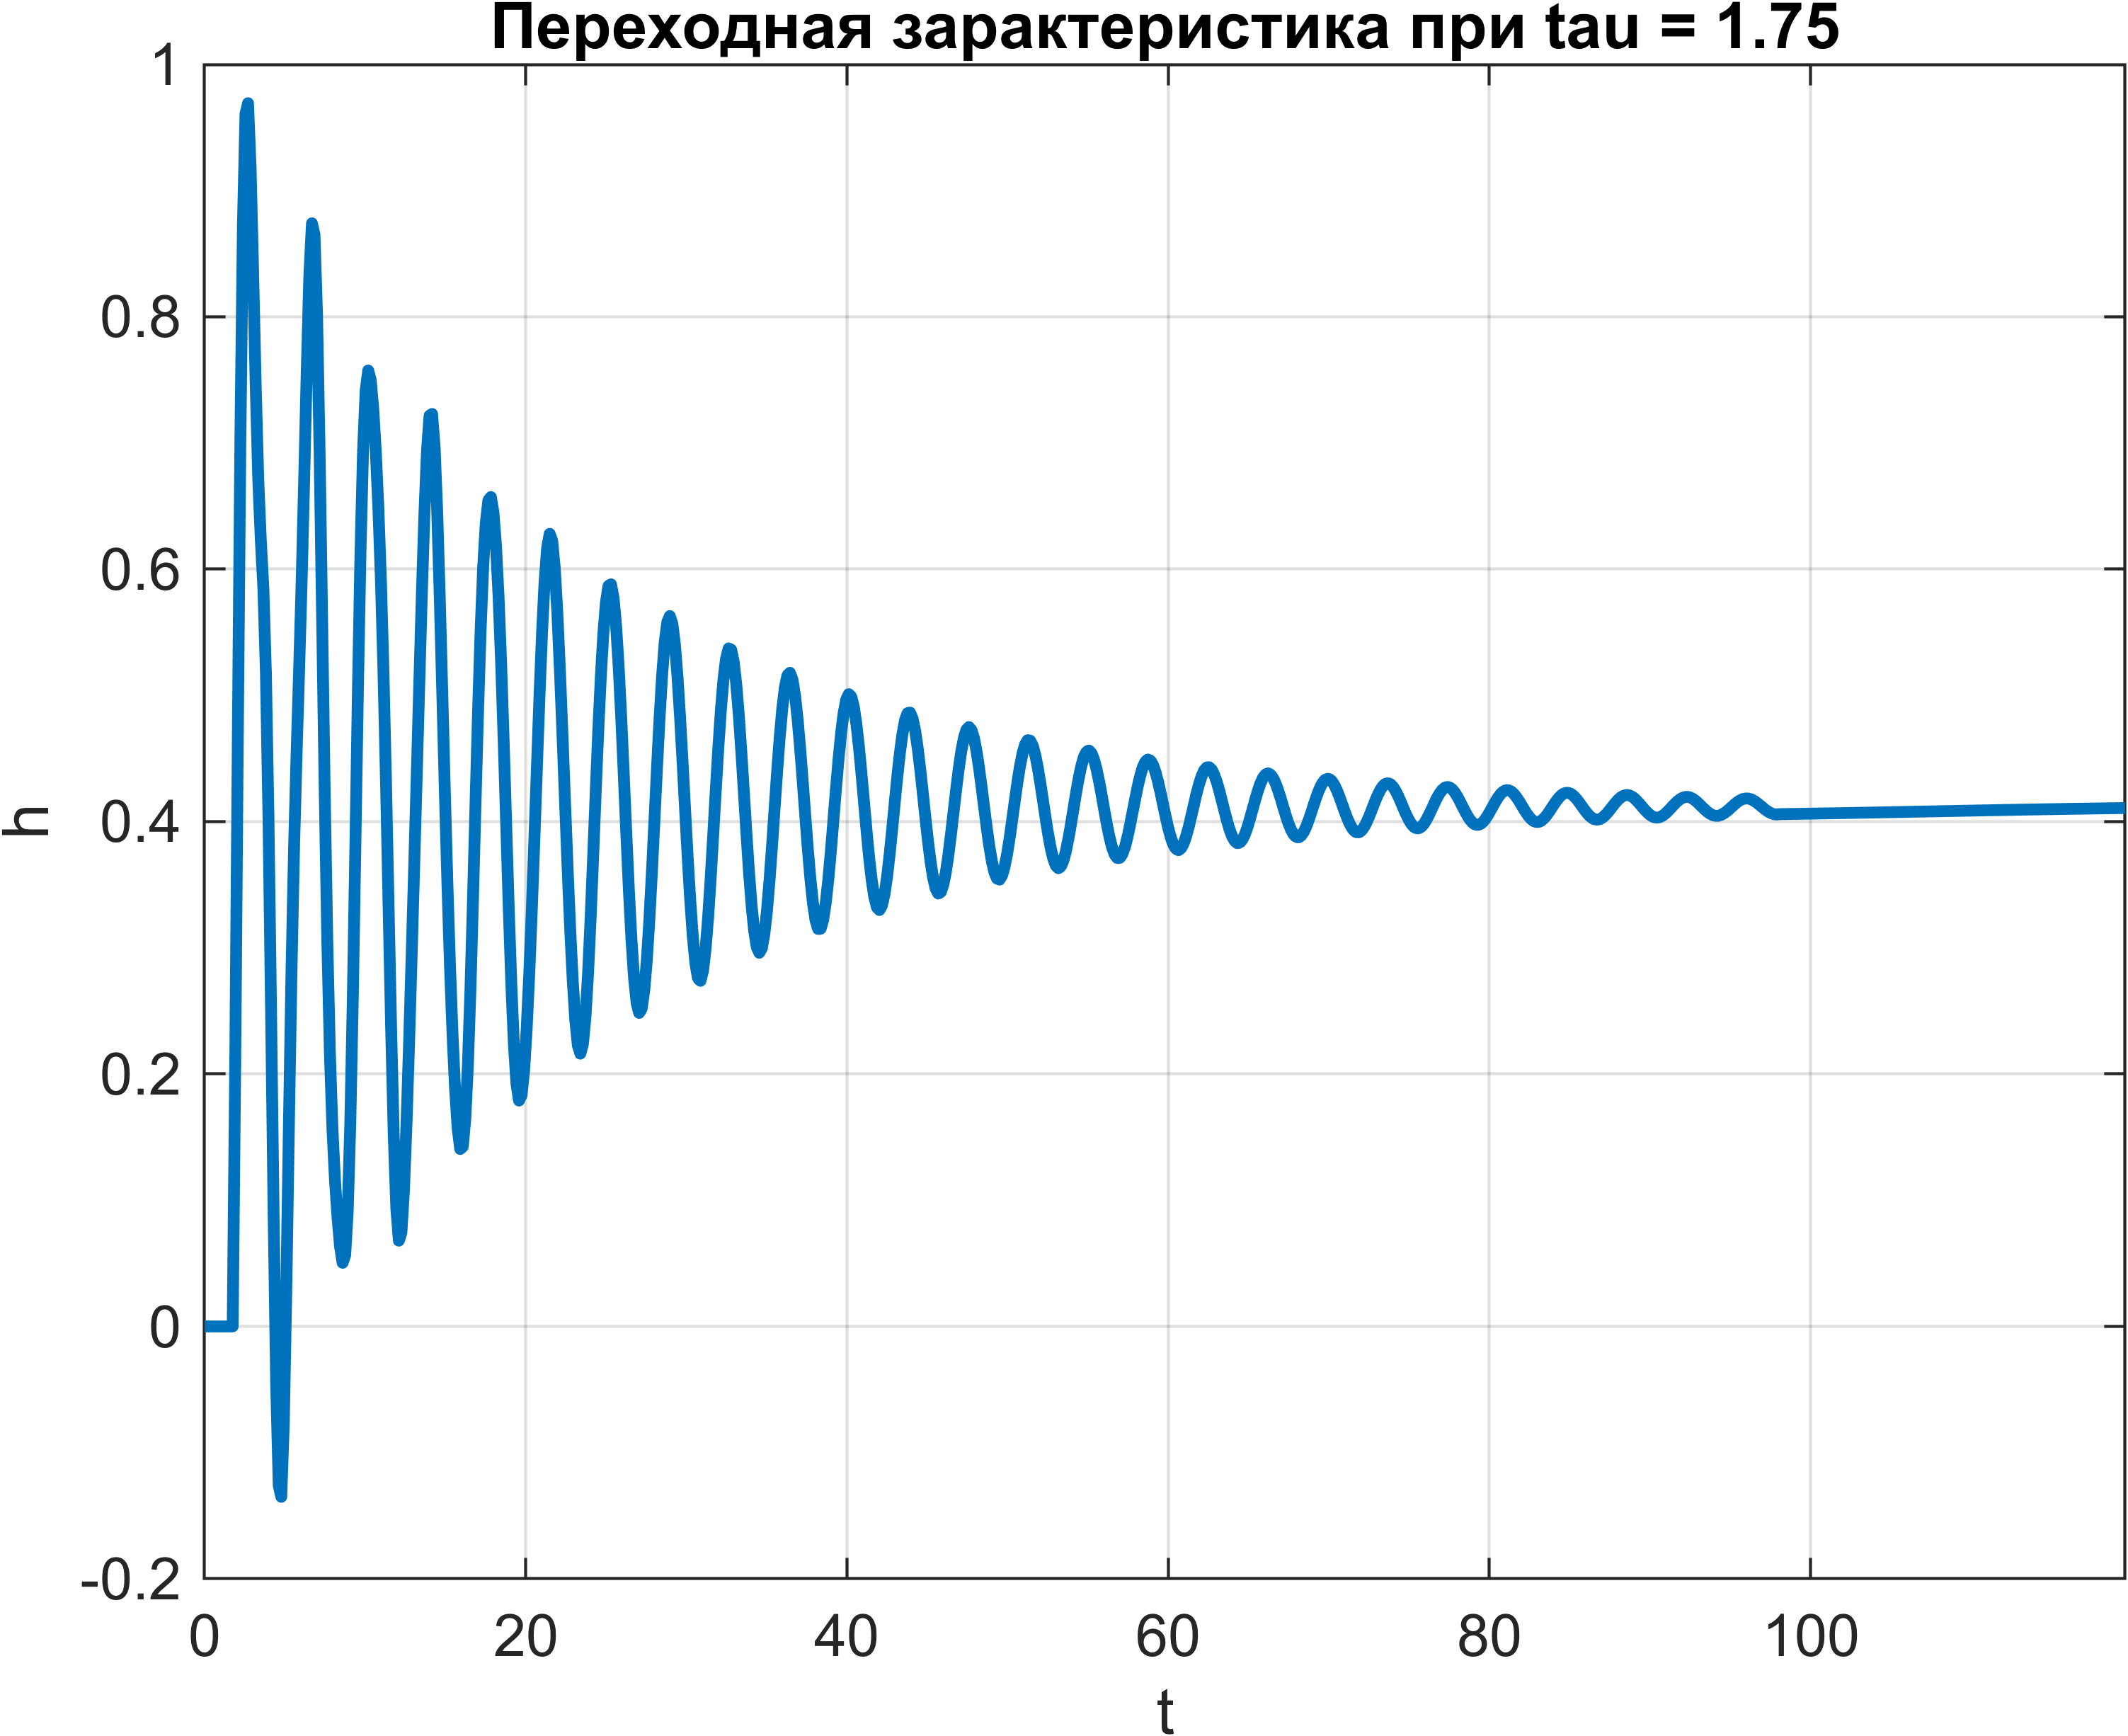
\includegraphics[width=\textwidth, trim={0cm 0cm 0cm 0cm}]{../images/3_1_7_cl.png}
    \end{minipage}
    \hfill
    \begin{minipage}{0.45\textwidth}
        \centering
        % Пустое место для 4-го элемента
    \end{minipage}
    \caption{Переходные характеристики системы для $\tau = 0.05$, $\tau = 1$, $\tau = 5$}
\end{figure}

\section{Передаточная функция $W_4(s)$}

Построим годограф Найквиста для передаточных функций с различными значениями запаздывания $\tau$:
\begin{enumerate}
    \item $\tau = 0$:
    \item $\tau = 0.5$:
    \item $\tau = 0.05$:
    \item $\tau = 1$:
    \item $\tau = 5$:
\end{enumerate}

\begin{figure}[H]
    \centering
    \centering
    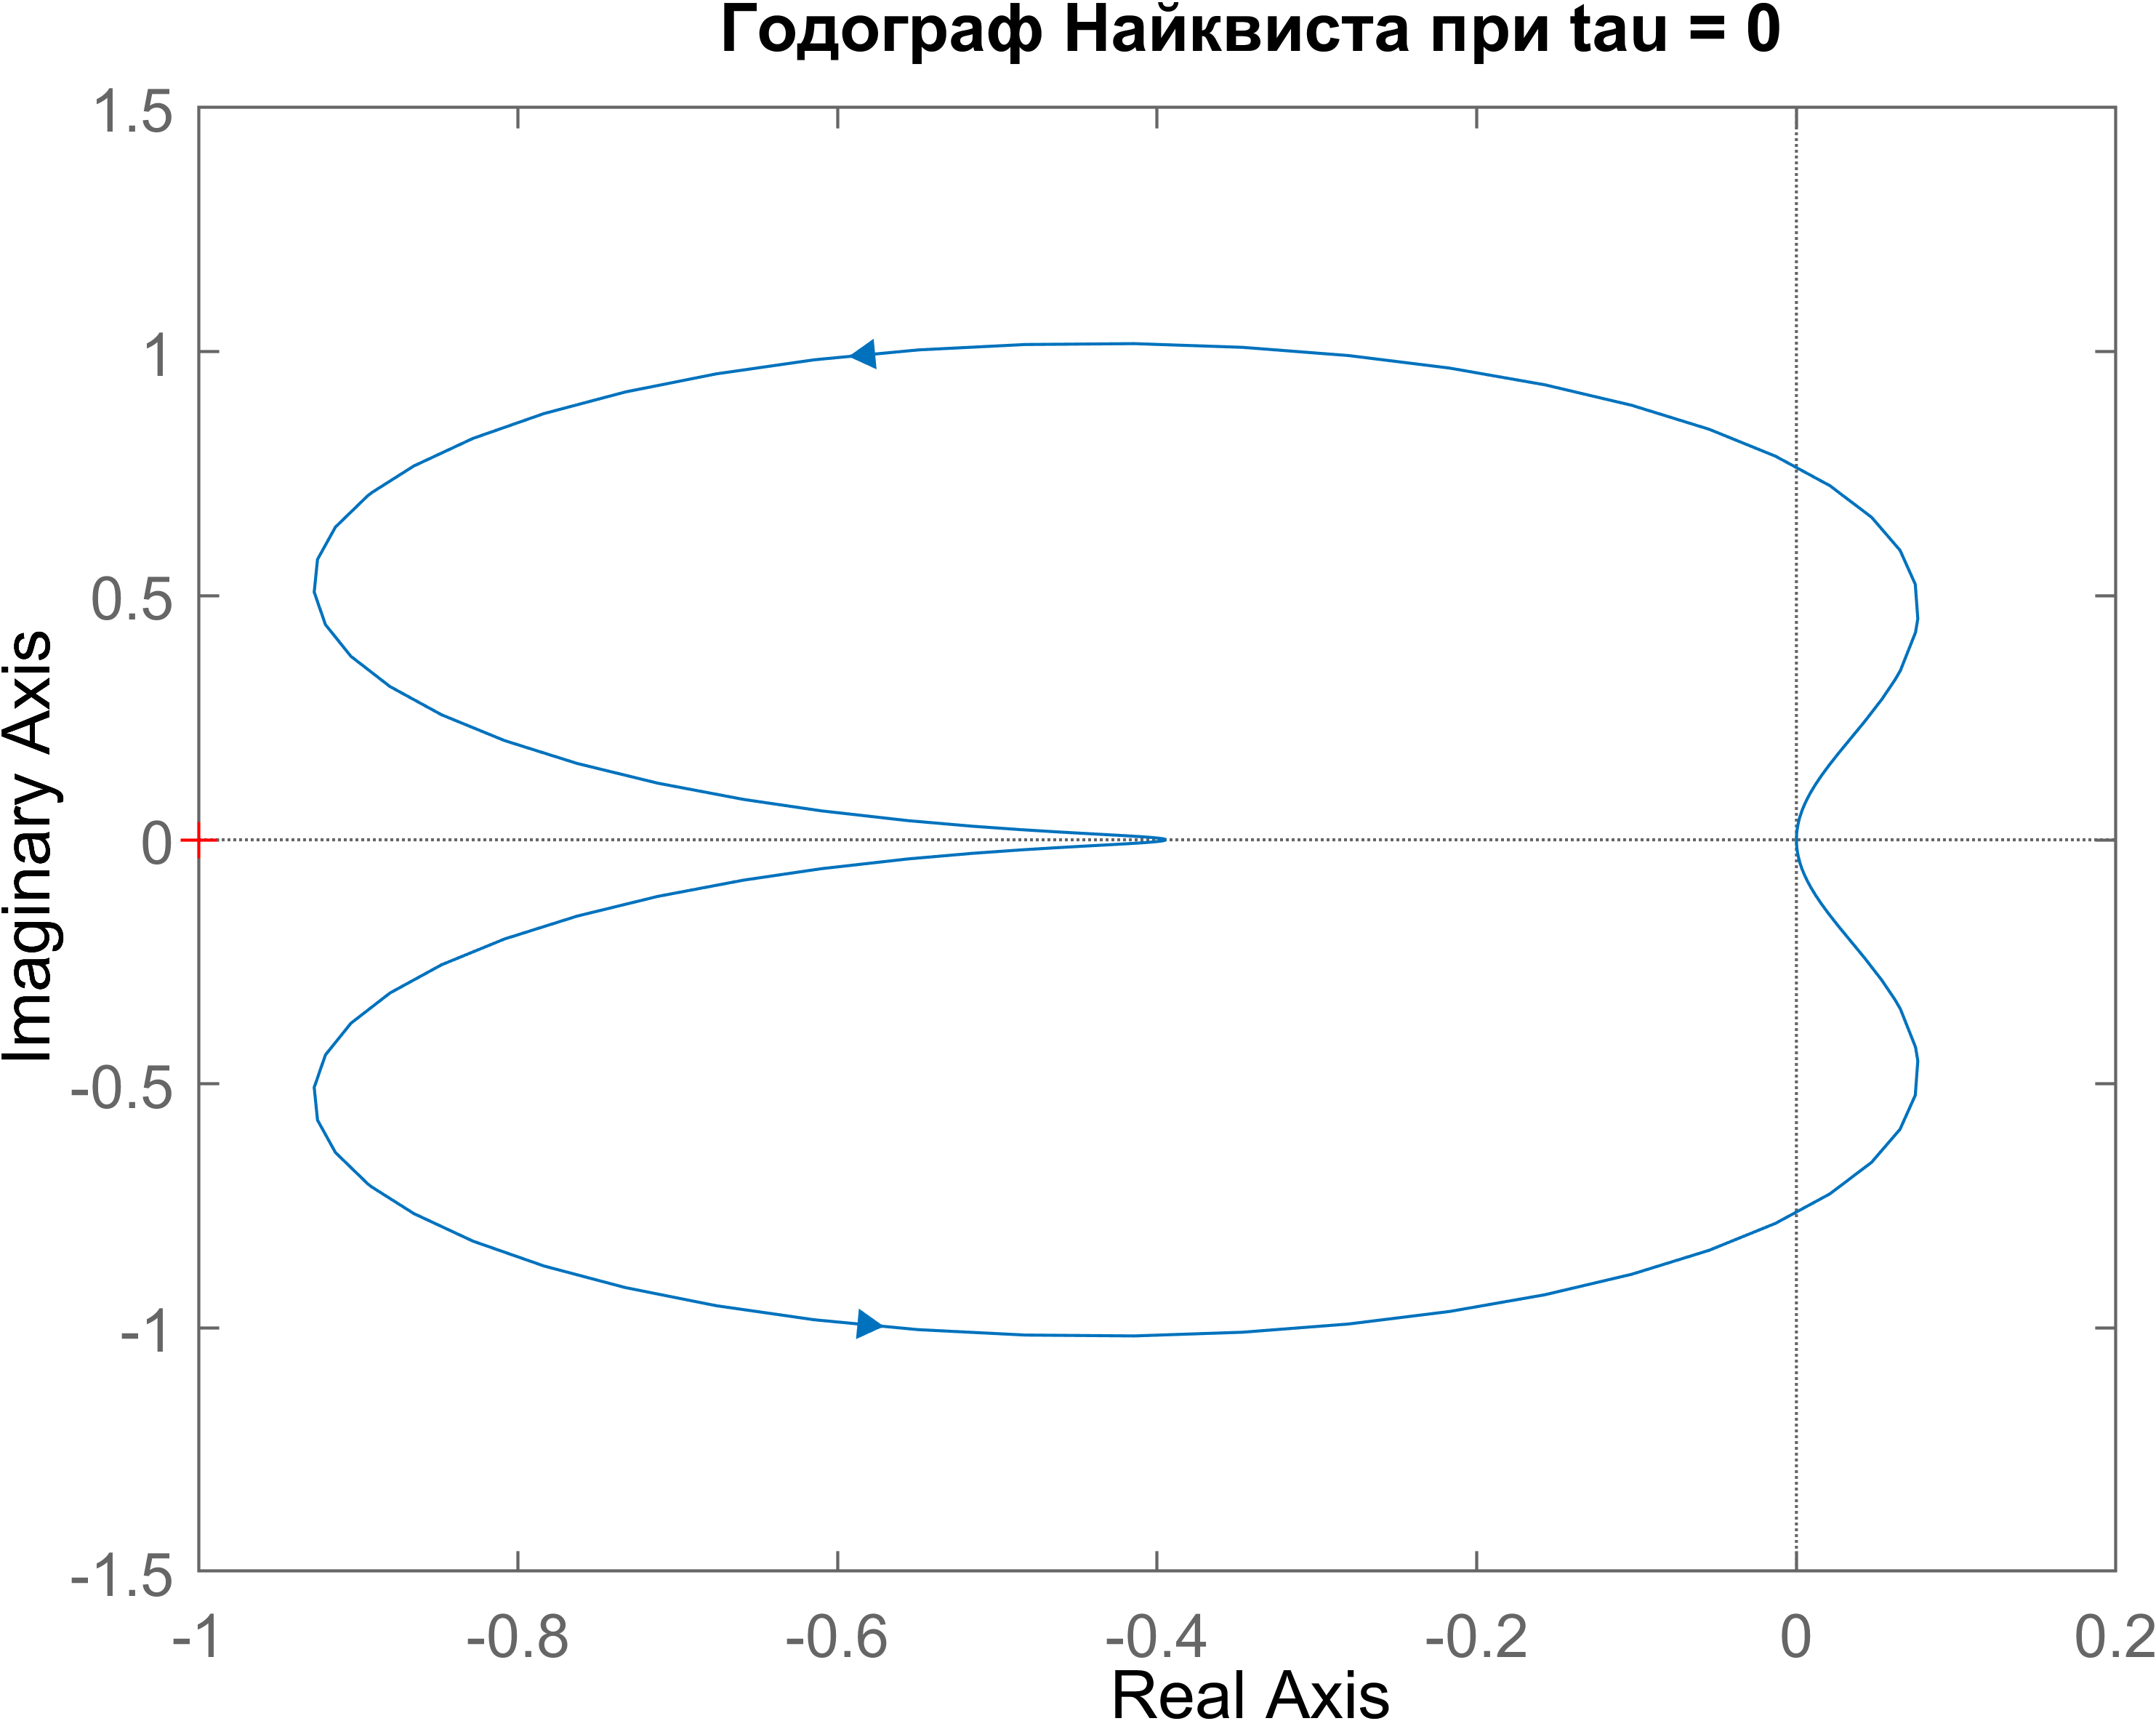
\includegraphics[width=0.7\textwidth, trim={0cm 0cm 0cm 0cm}]{../images/3_2_0_hod.png}
    \caption{Годограф Найквиста для $\tau = 0$}
\end{figure}

\begin{figure}[H]
    \centering
    \centering
    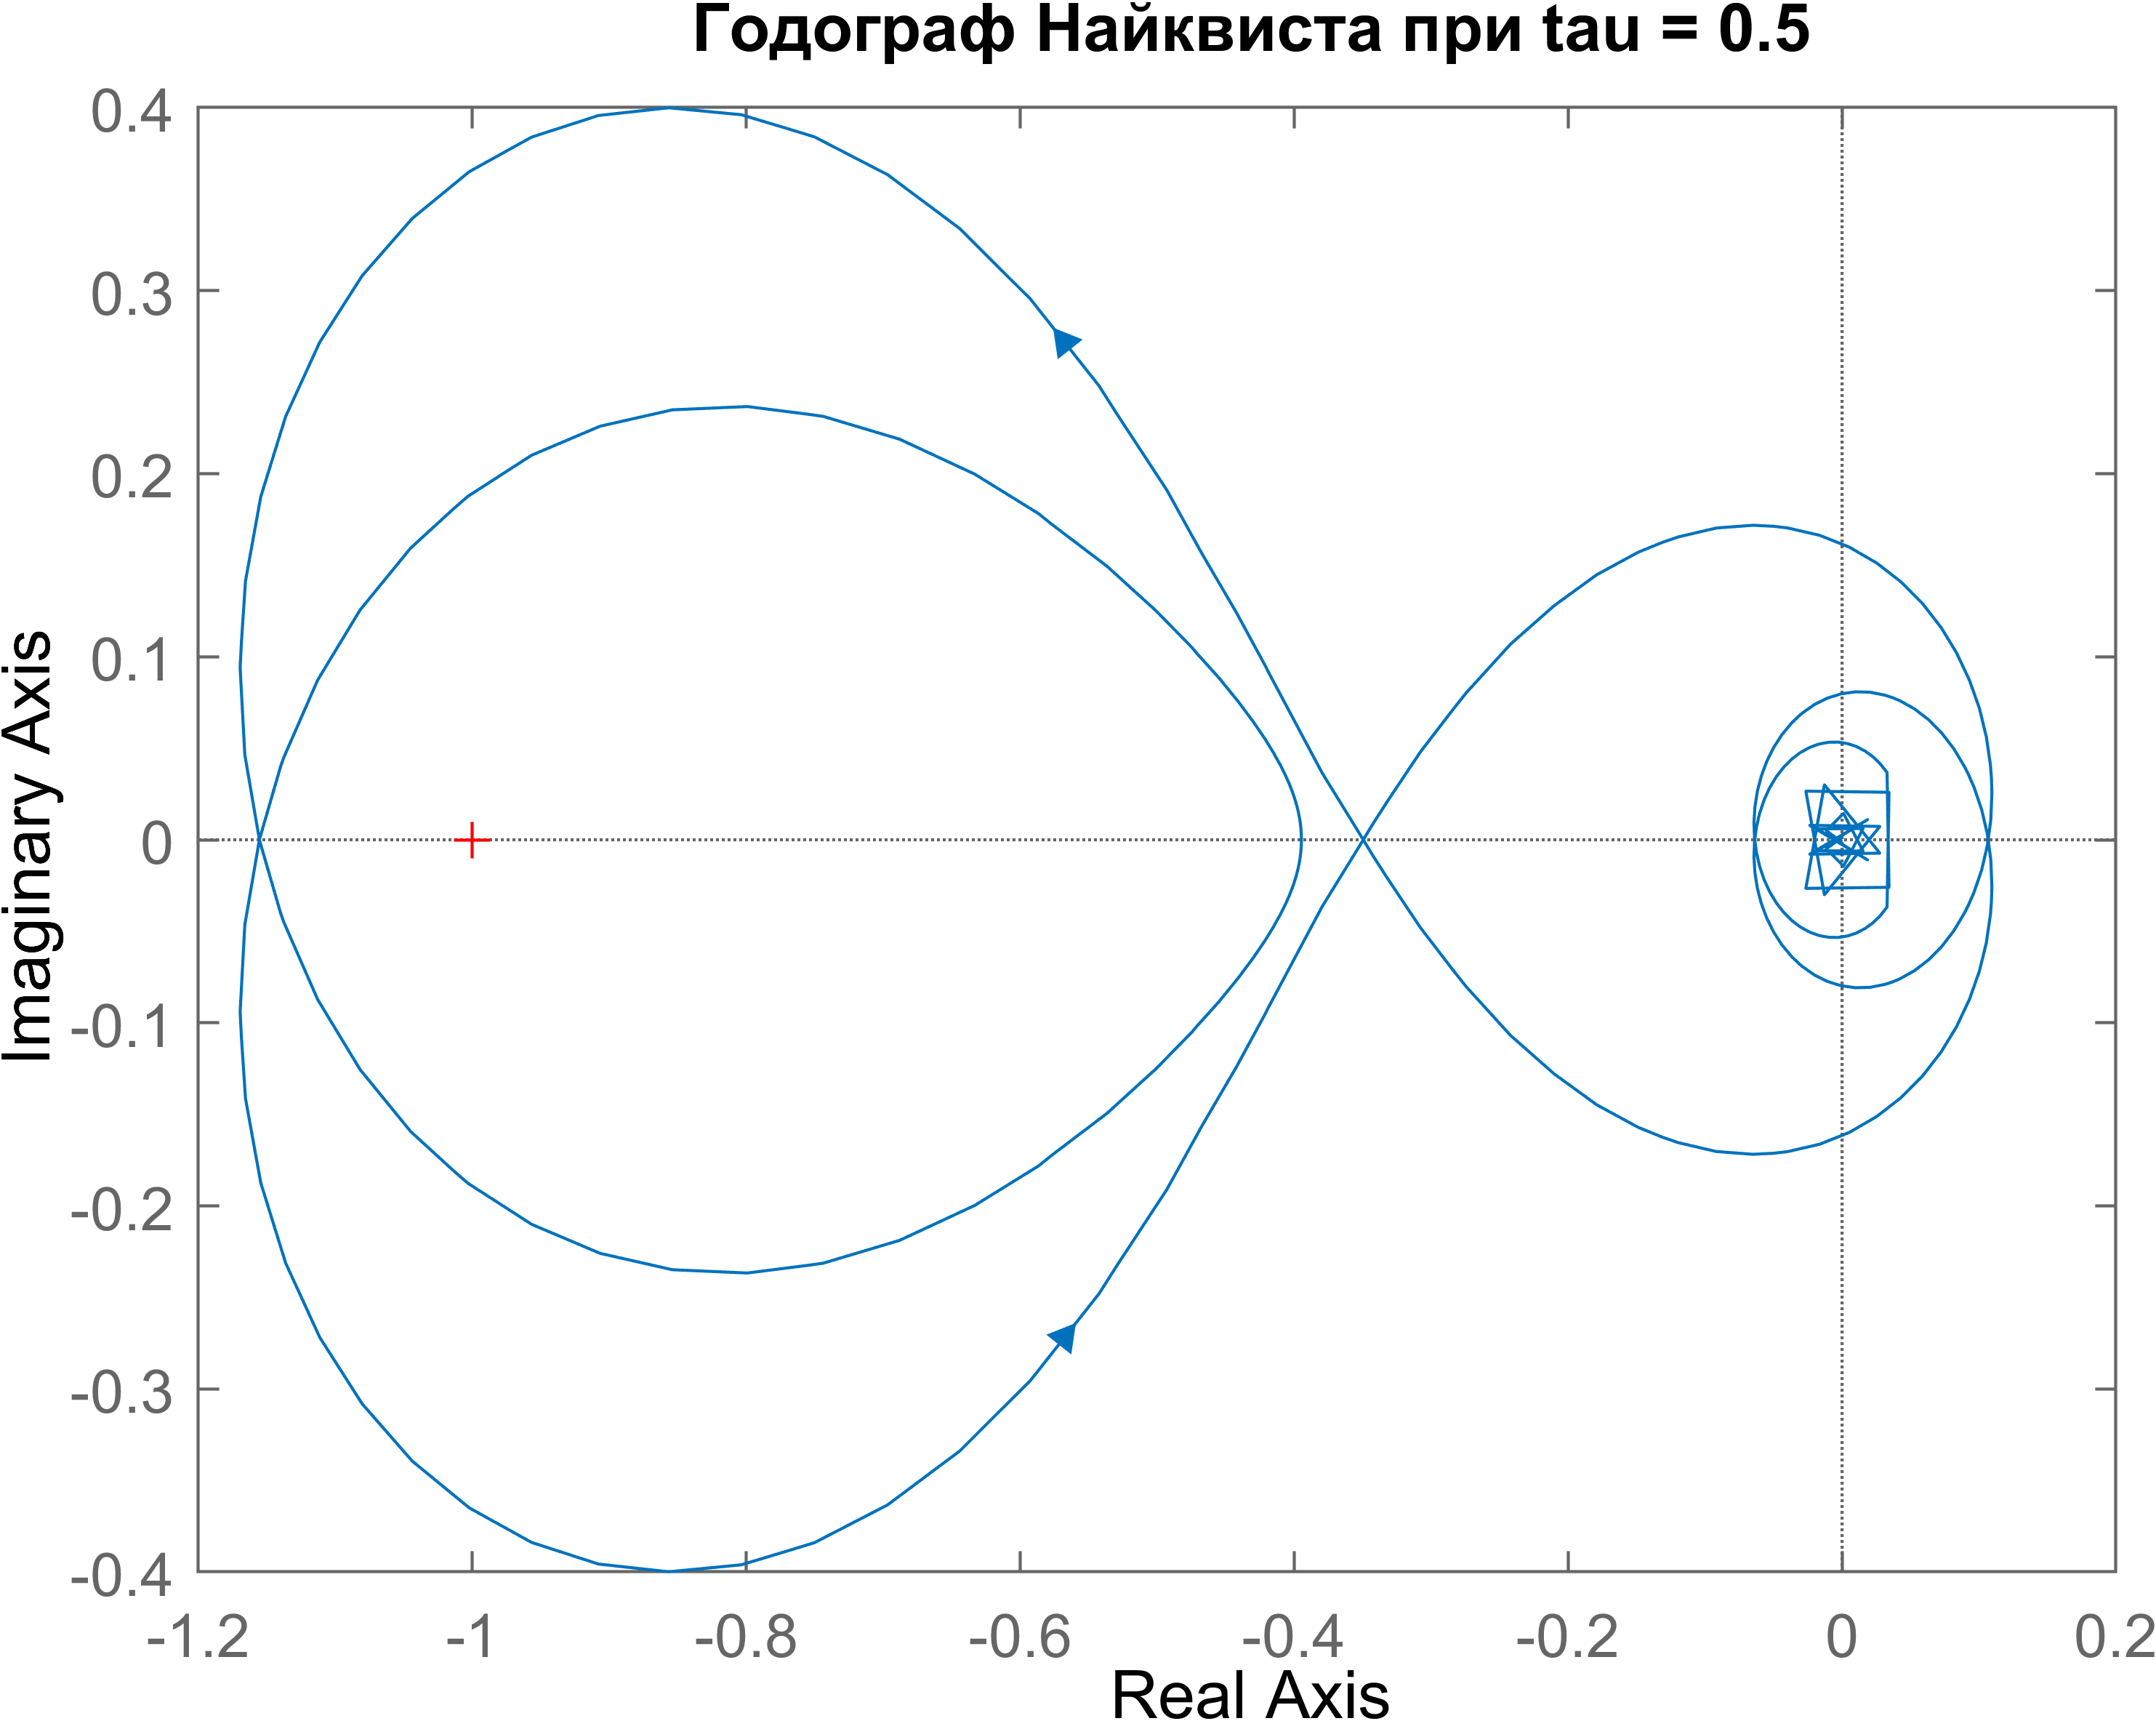
\includegraphics[width=0.7\textwidth, trim={0cm 0cm 0cm 0cm}]{../images/3_2_1_hod.png}
    \caption{Годограф Найквиста для $\tau = 0.5$}
\end{figure}

\begin{figure}[H]
    \centering
    \centering
    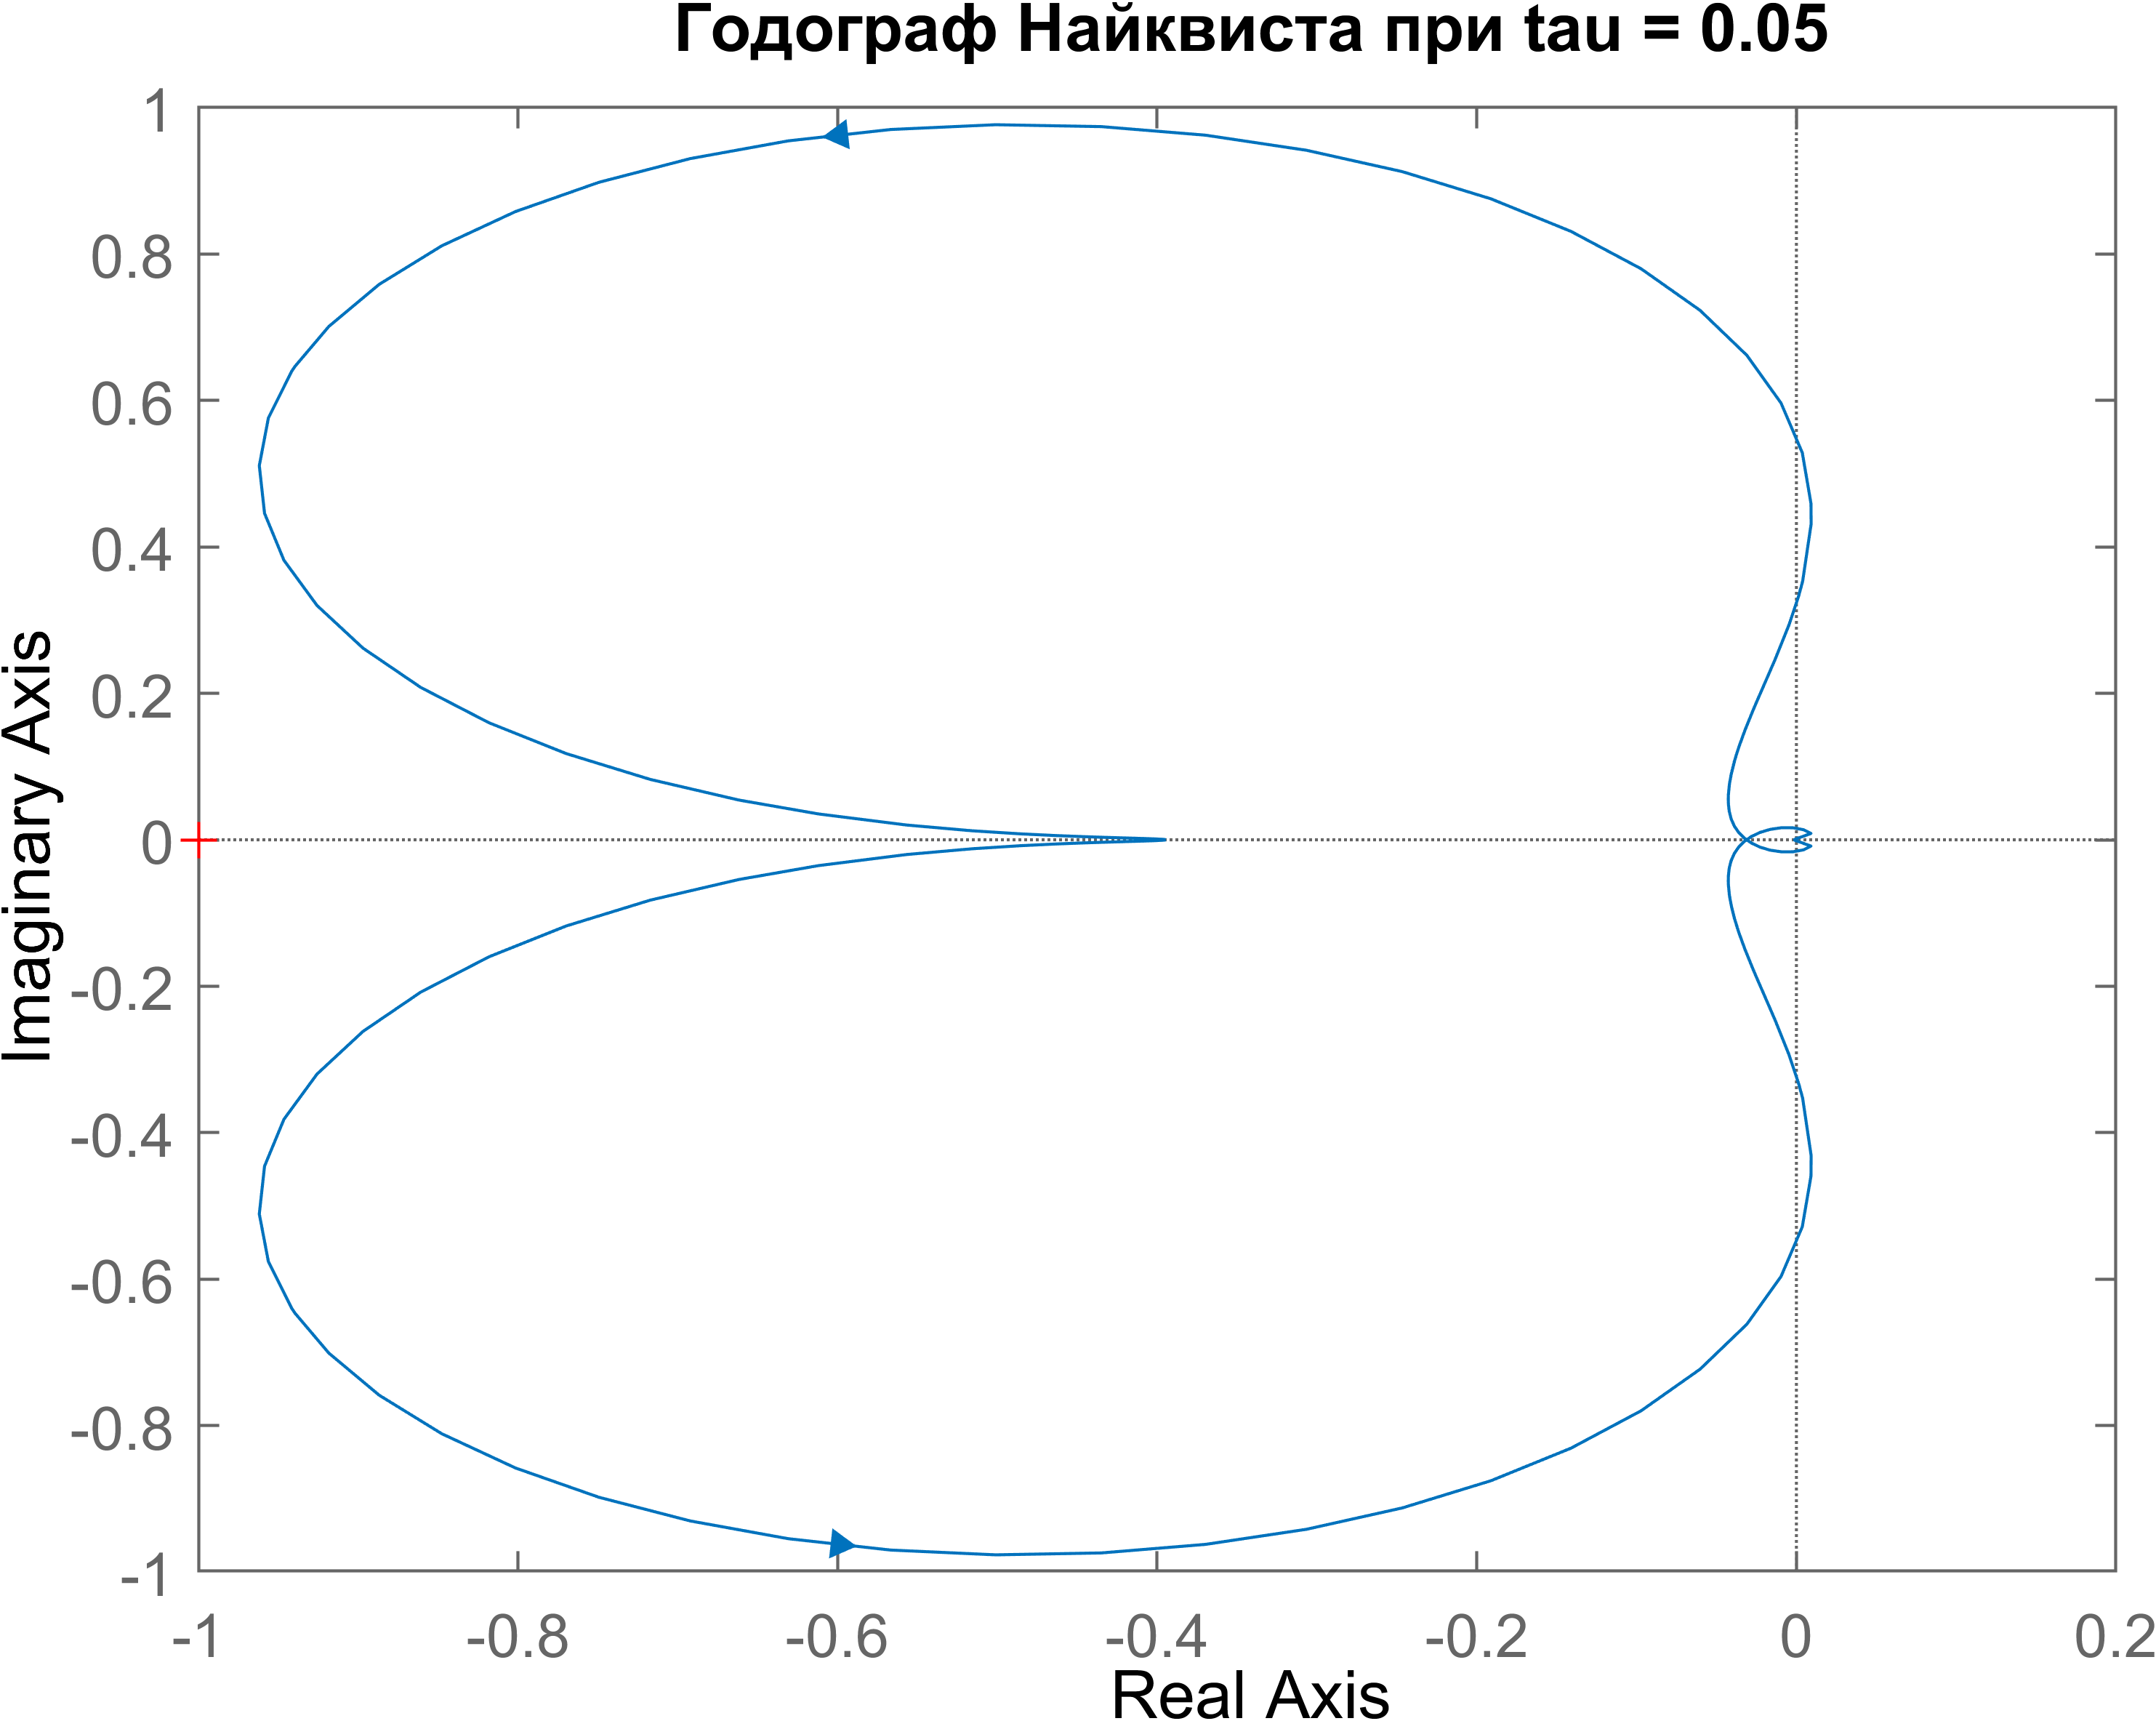
\includegraphics[width=0.7\textwidth, trim={0cm 0cm 0cm 0cm}]{../images/3_2_2_hod.png}
    \caption{Годограф Найквиста для $\tau = 0.05$}
\end{figure}

\begin{figure}[H]
    \centering
    \centering
    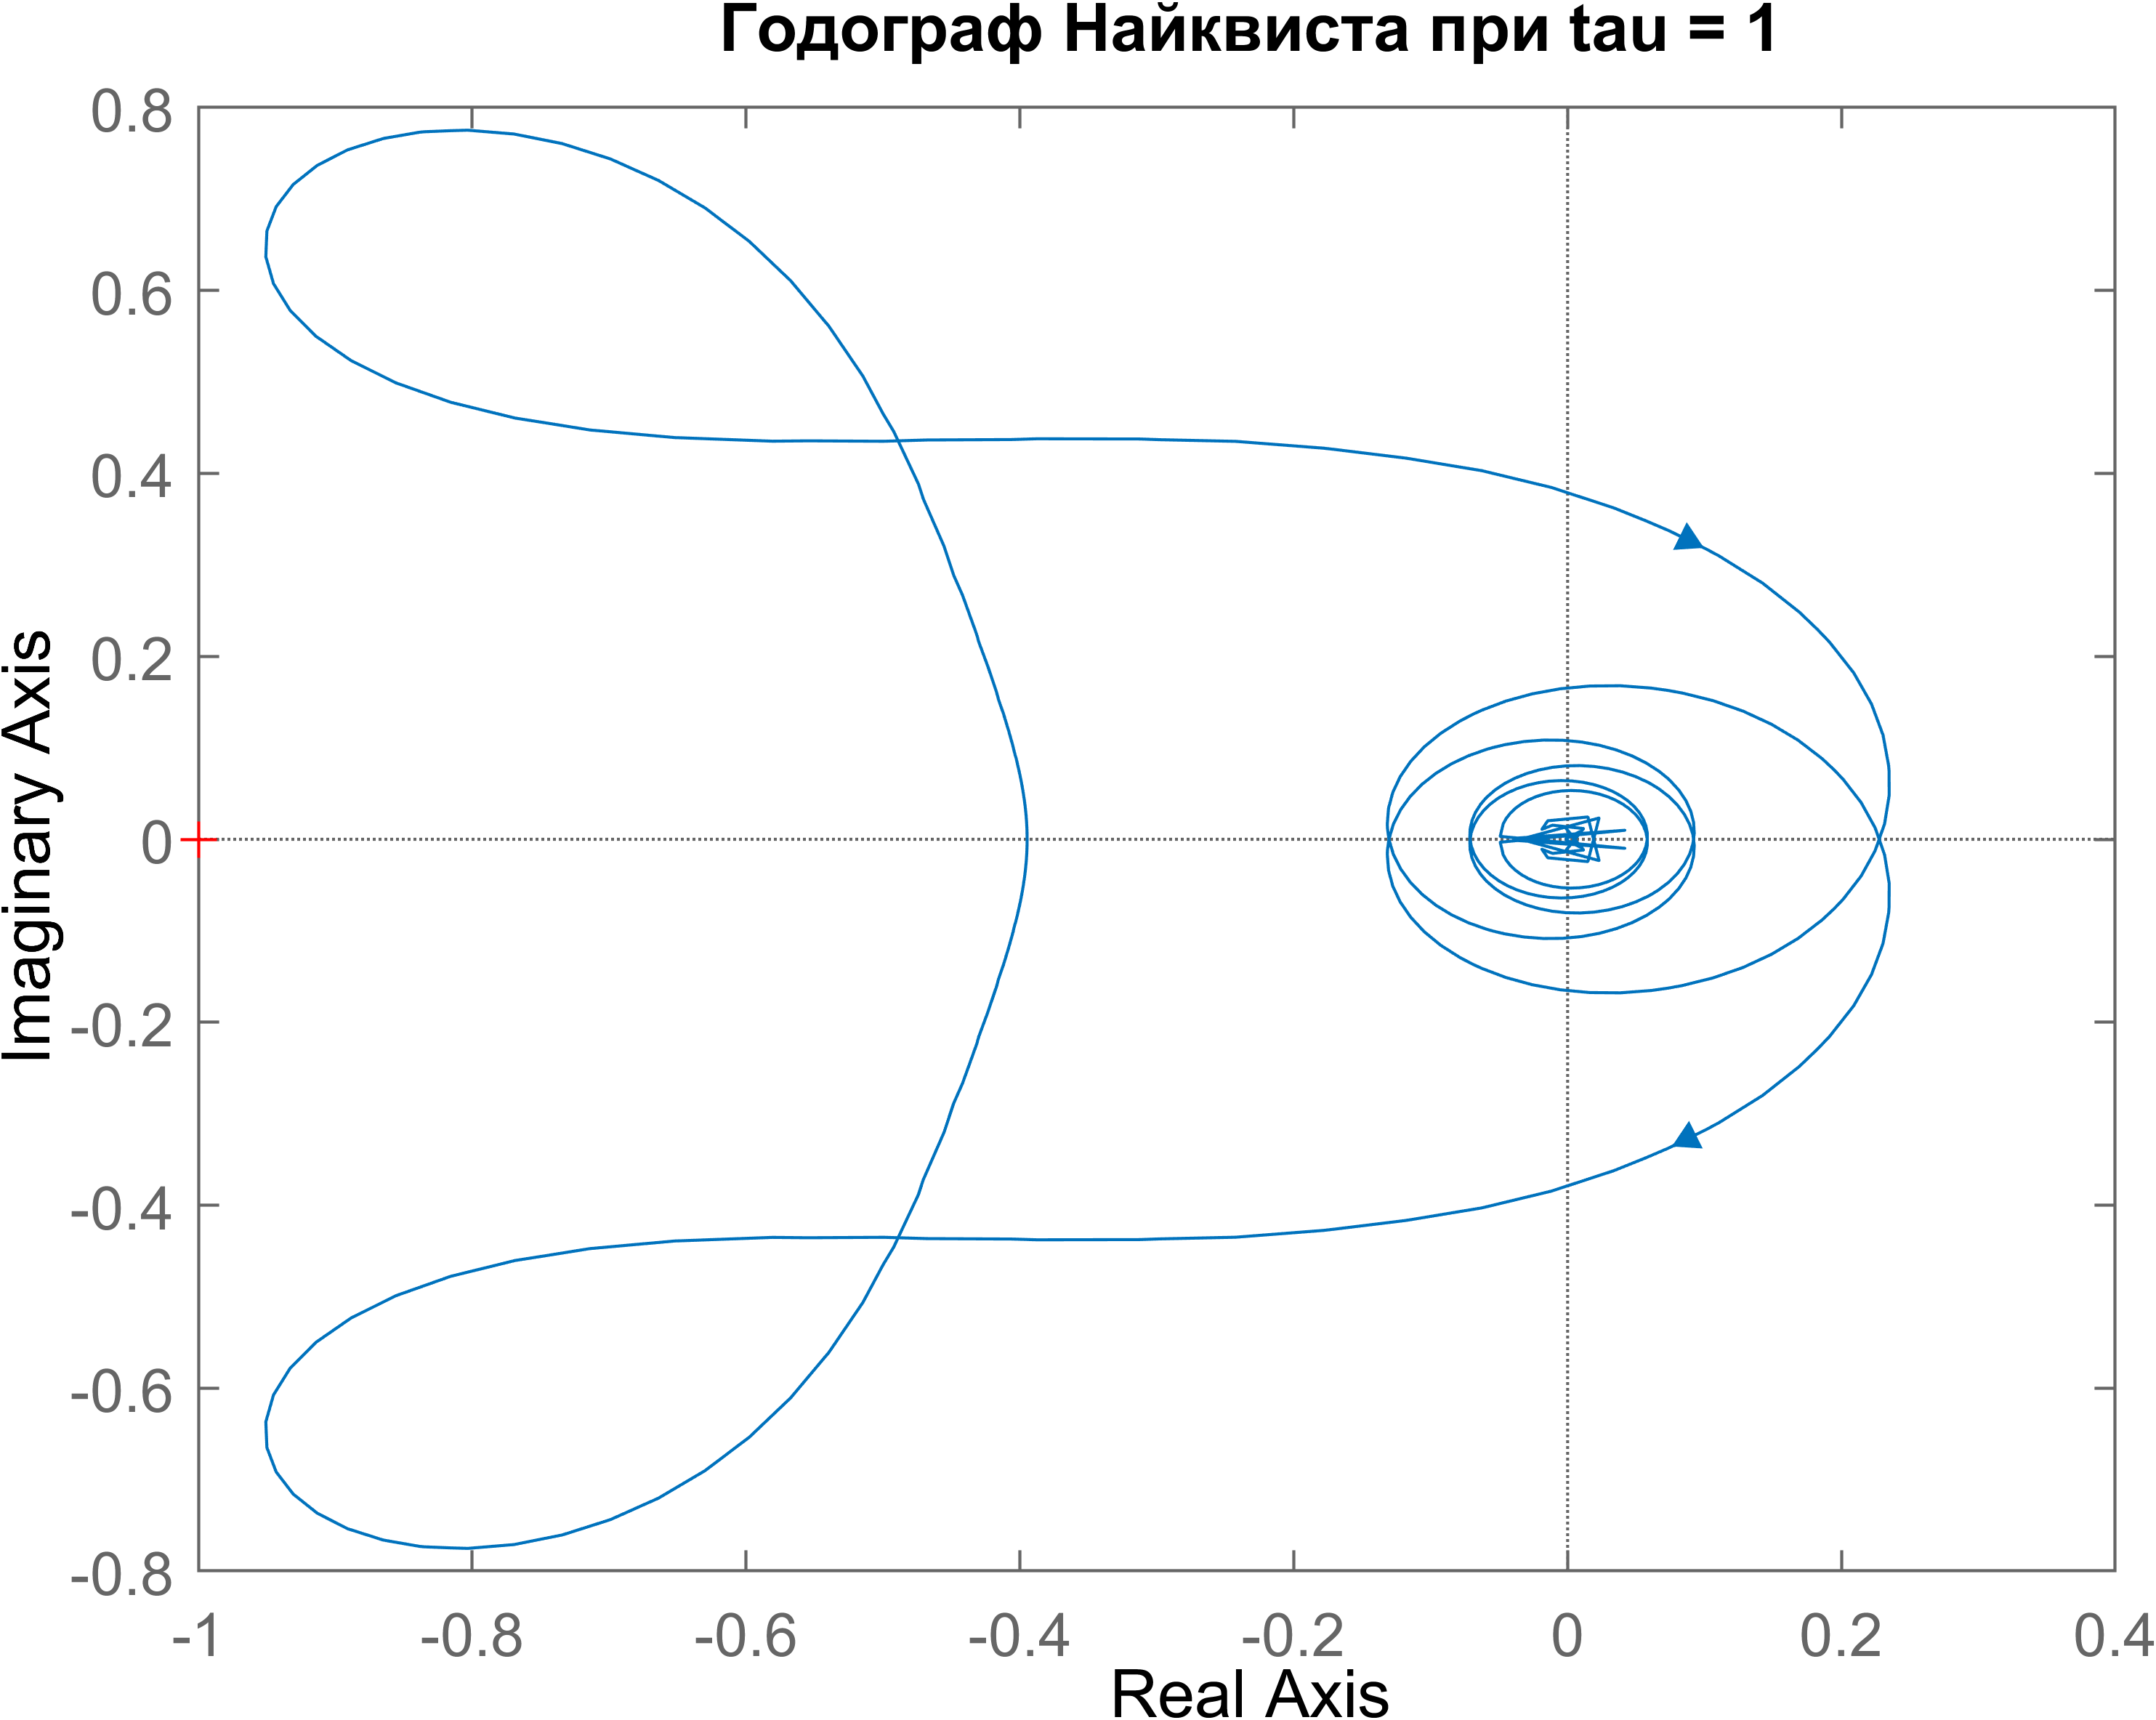
\includegraphics[width=0.7\textwidth, trim={0cm 0cm 0cm 0cm}]{../images/3_2_3_hod.png}
    \caption{Годограф Найквиста для $\tau = 1$}
\end{figure}

\begin{figure}[H]
    \centering
    \centering
    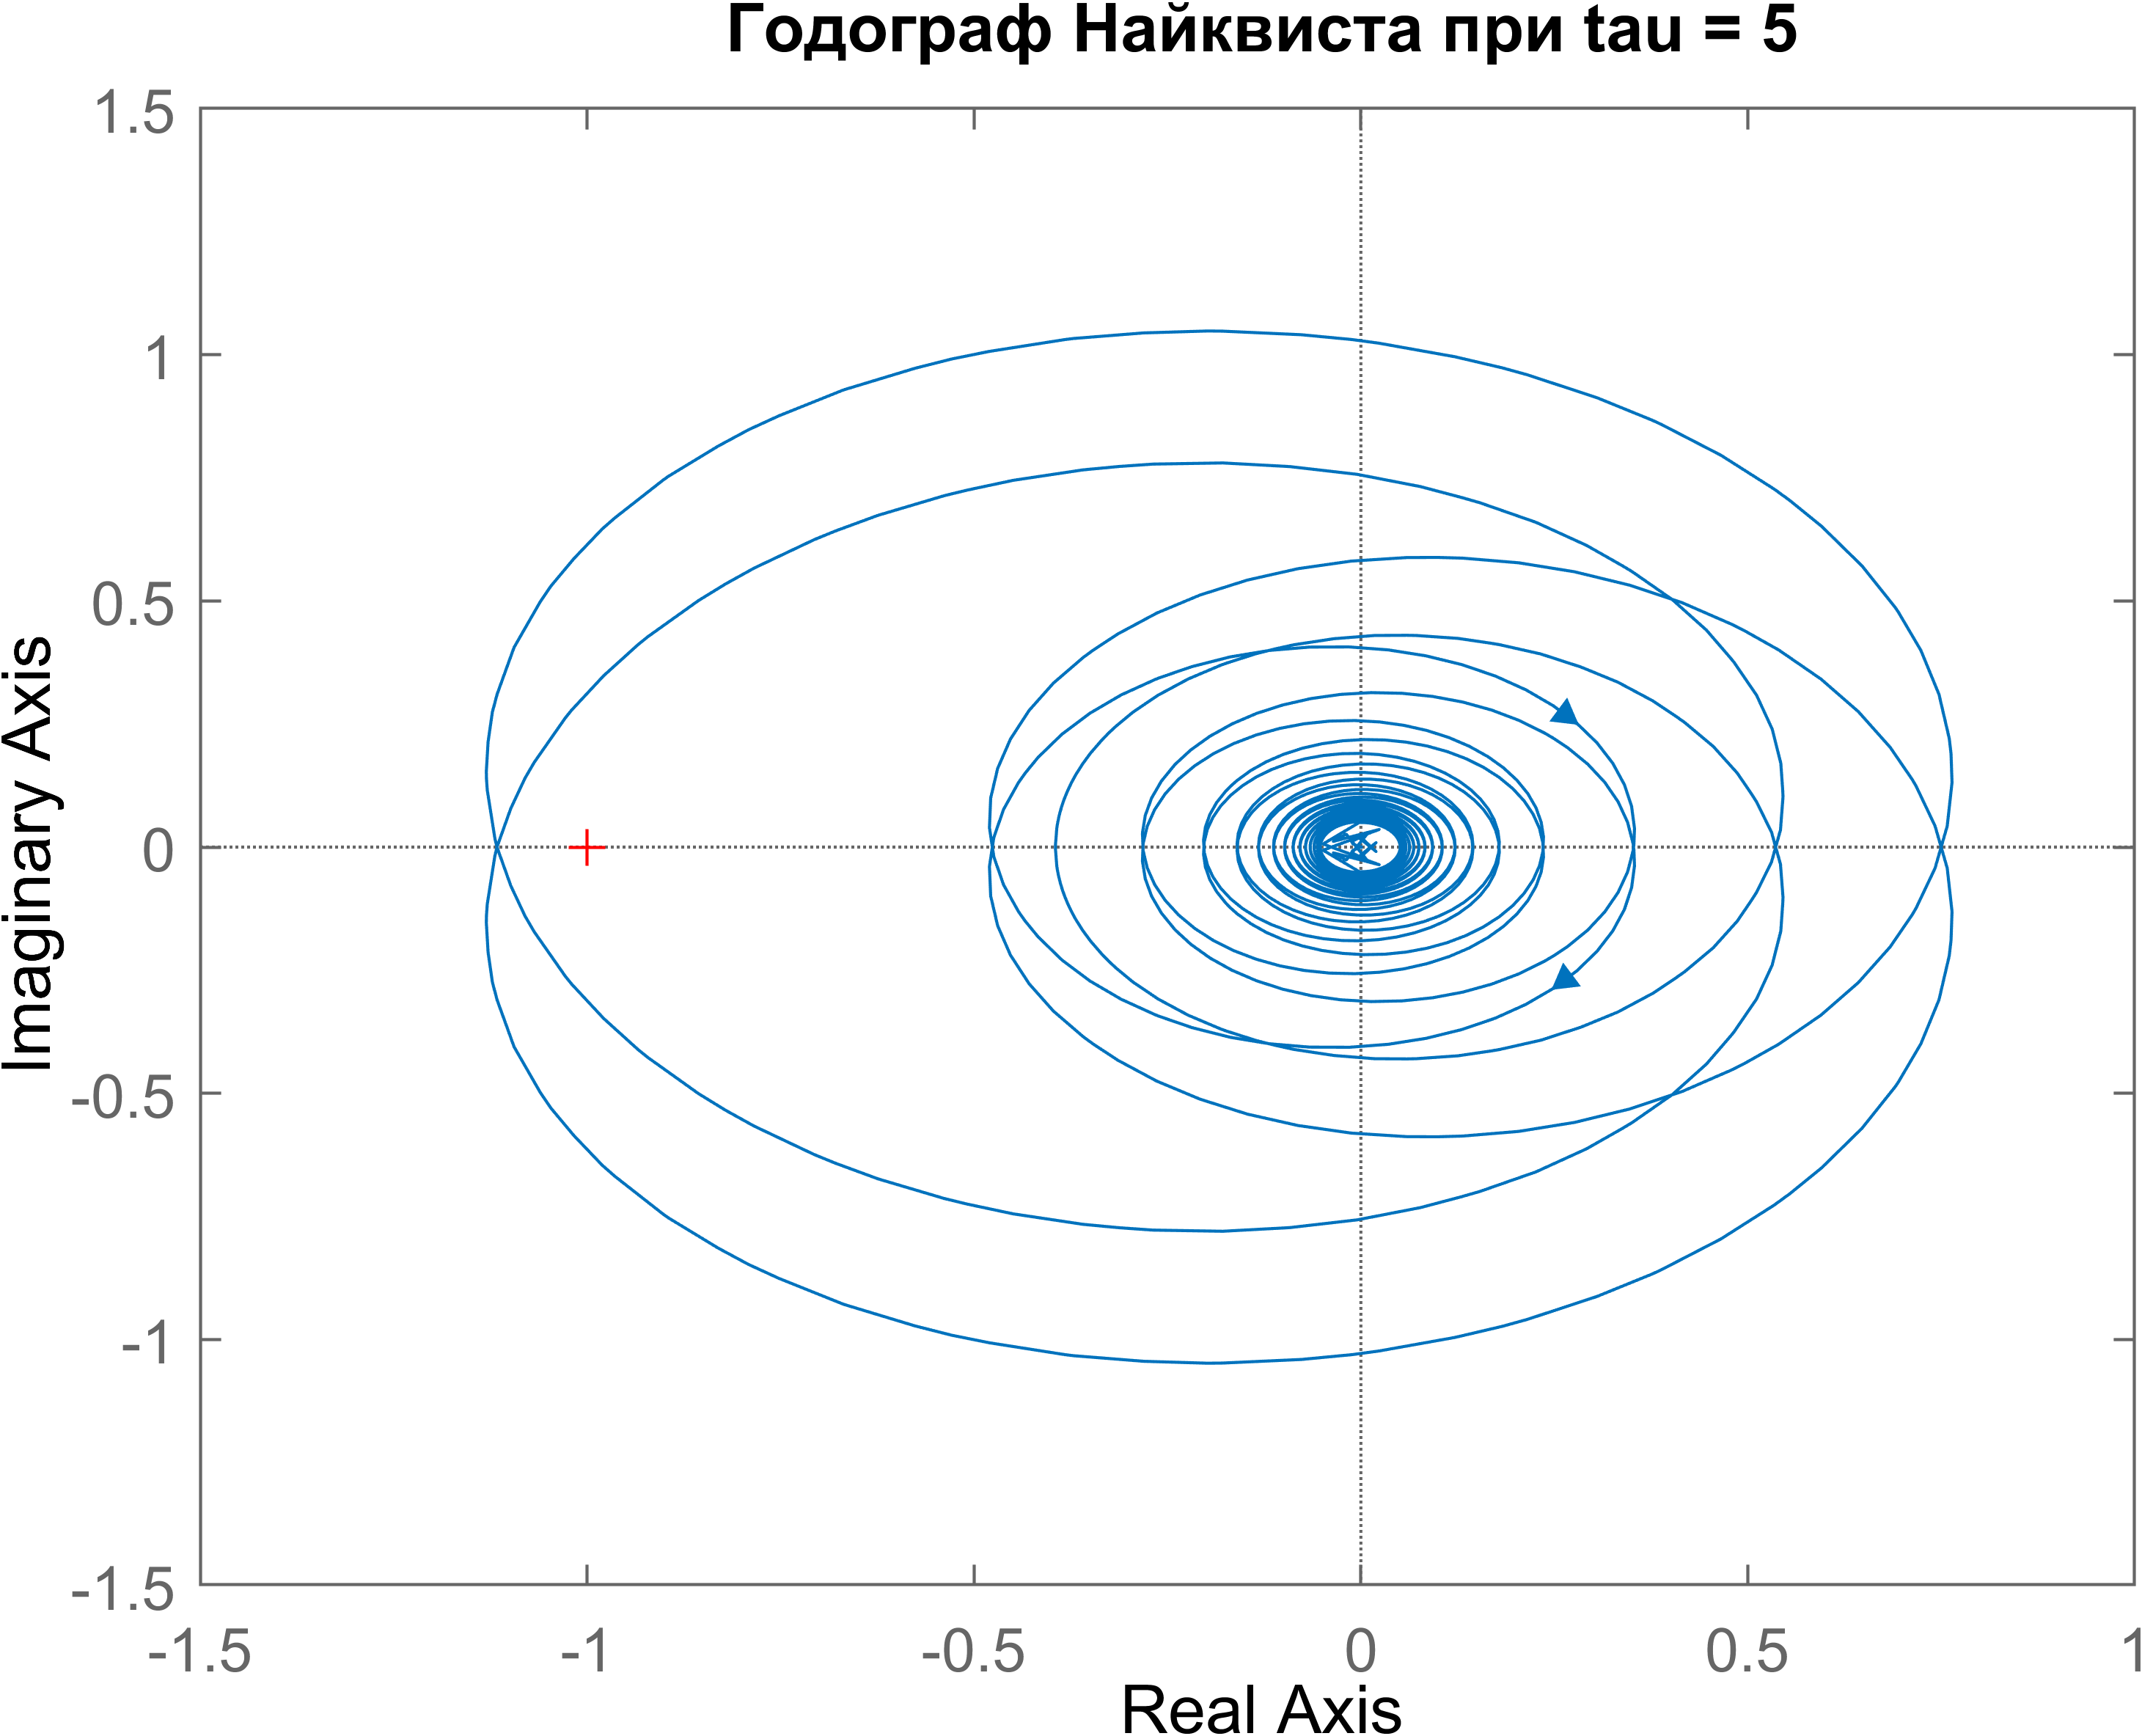
\includegraphics[width=0.7\textwidth, trim={0cm 0cm 0cm 0cm}]{../images/3_2_4_hod.png}
    \caption{Годограф Найквиста для $\tau = 5$}
\end{figure}

Как видим эта передаточная функция ведет себя похожим образом, что и предыдущая. При увеличении запаздывания $\tau$ годограф все 
больше закручивается. У этой системы расположение корней совпадает с предыдущей, поэтому граничные значения запаздывания найдем
аналогично:
\[
w_{cp1} = 1.86
\]
\[
\varphi_{p1} = \pi + \varphi(w_{cp1}) = \pi - 1.81 = 1.33
\]
\[
\tau_1 = \frac{\varphi_{p1}}{w_{cp1}} = 0.72
\]


\[
w_{cp2} = 1.24
\]
\[
\varphi_{p2} = \pi + \varphi(w_{cp2}) = \pi - 2.62 = 0.52
\]
\[
\tau_2 = \frac{\varphi_{p2}}{w_{cp2}} = 0.42
\]

Таким образом, система остается устойчивой при $0.42 >\tau> 0.72$. Продемонстрируем переходные
характеристики системы при коэффициентах $\tau$, соответствующих устойчивости и неустойчивости для каждой из областей:

\begin{figure}[H]
    \centering
    \begin{minipage}{0.45\textwidth}
        \centering
        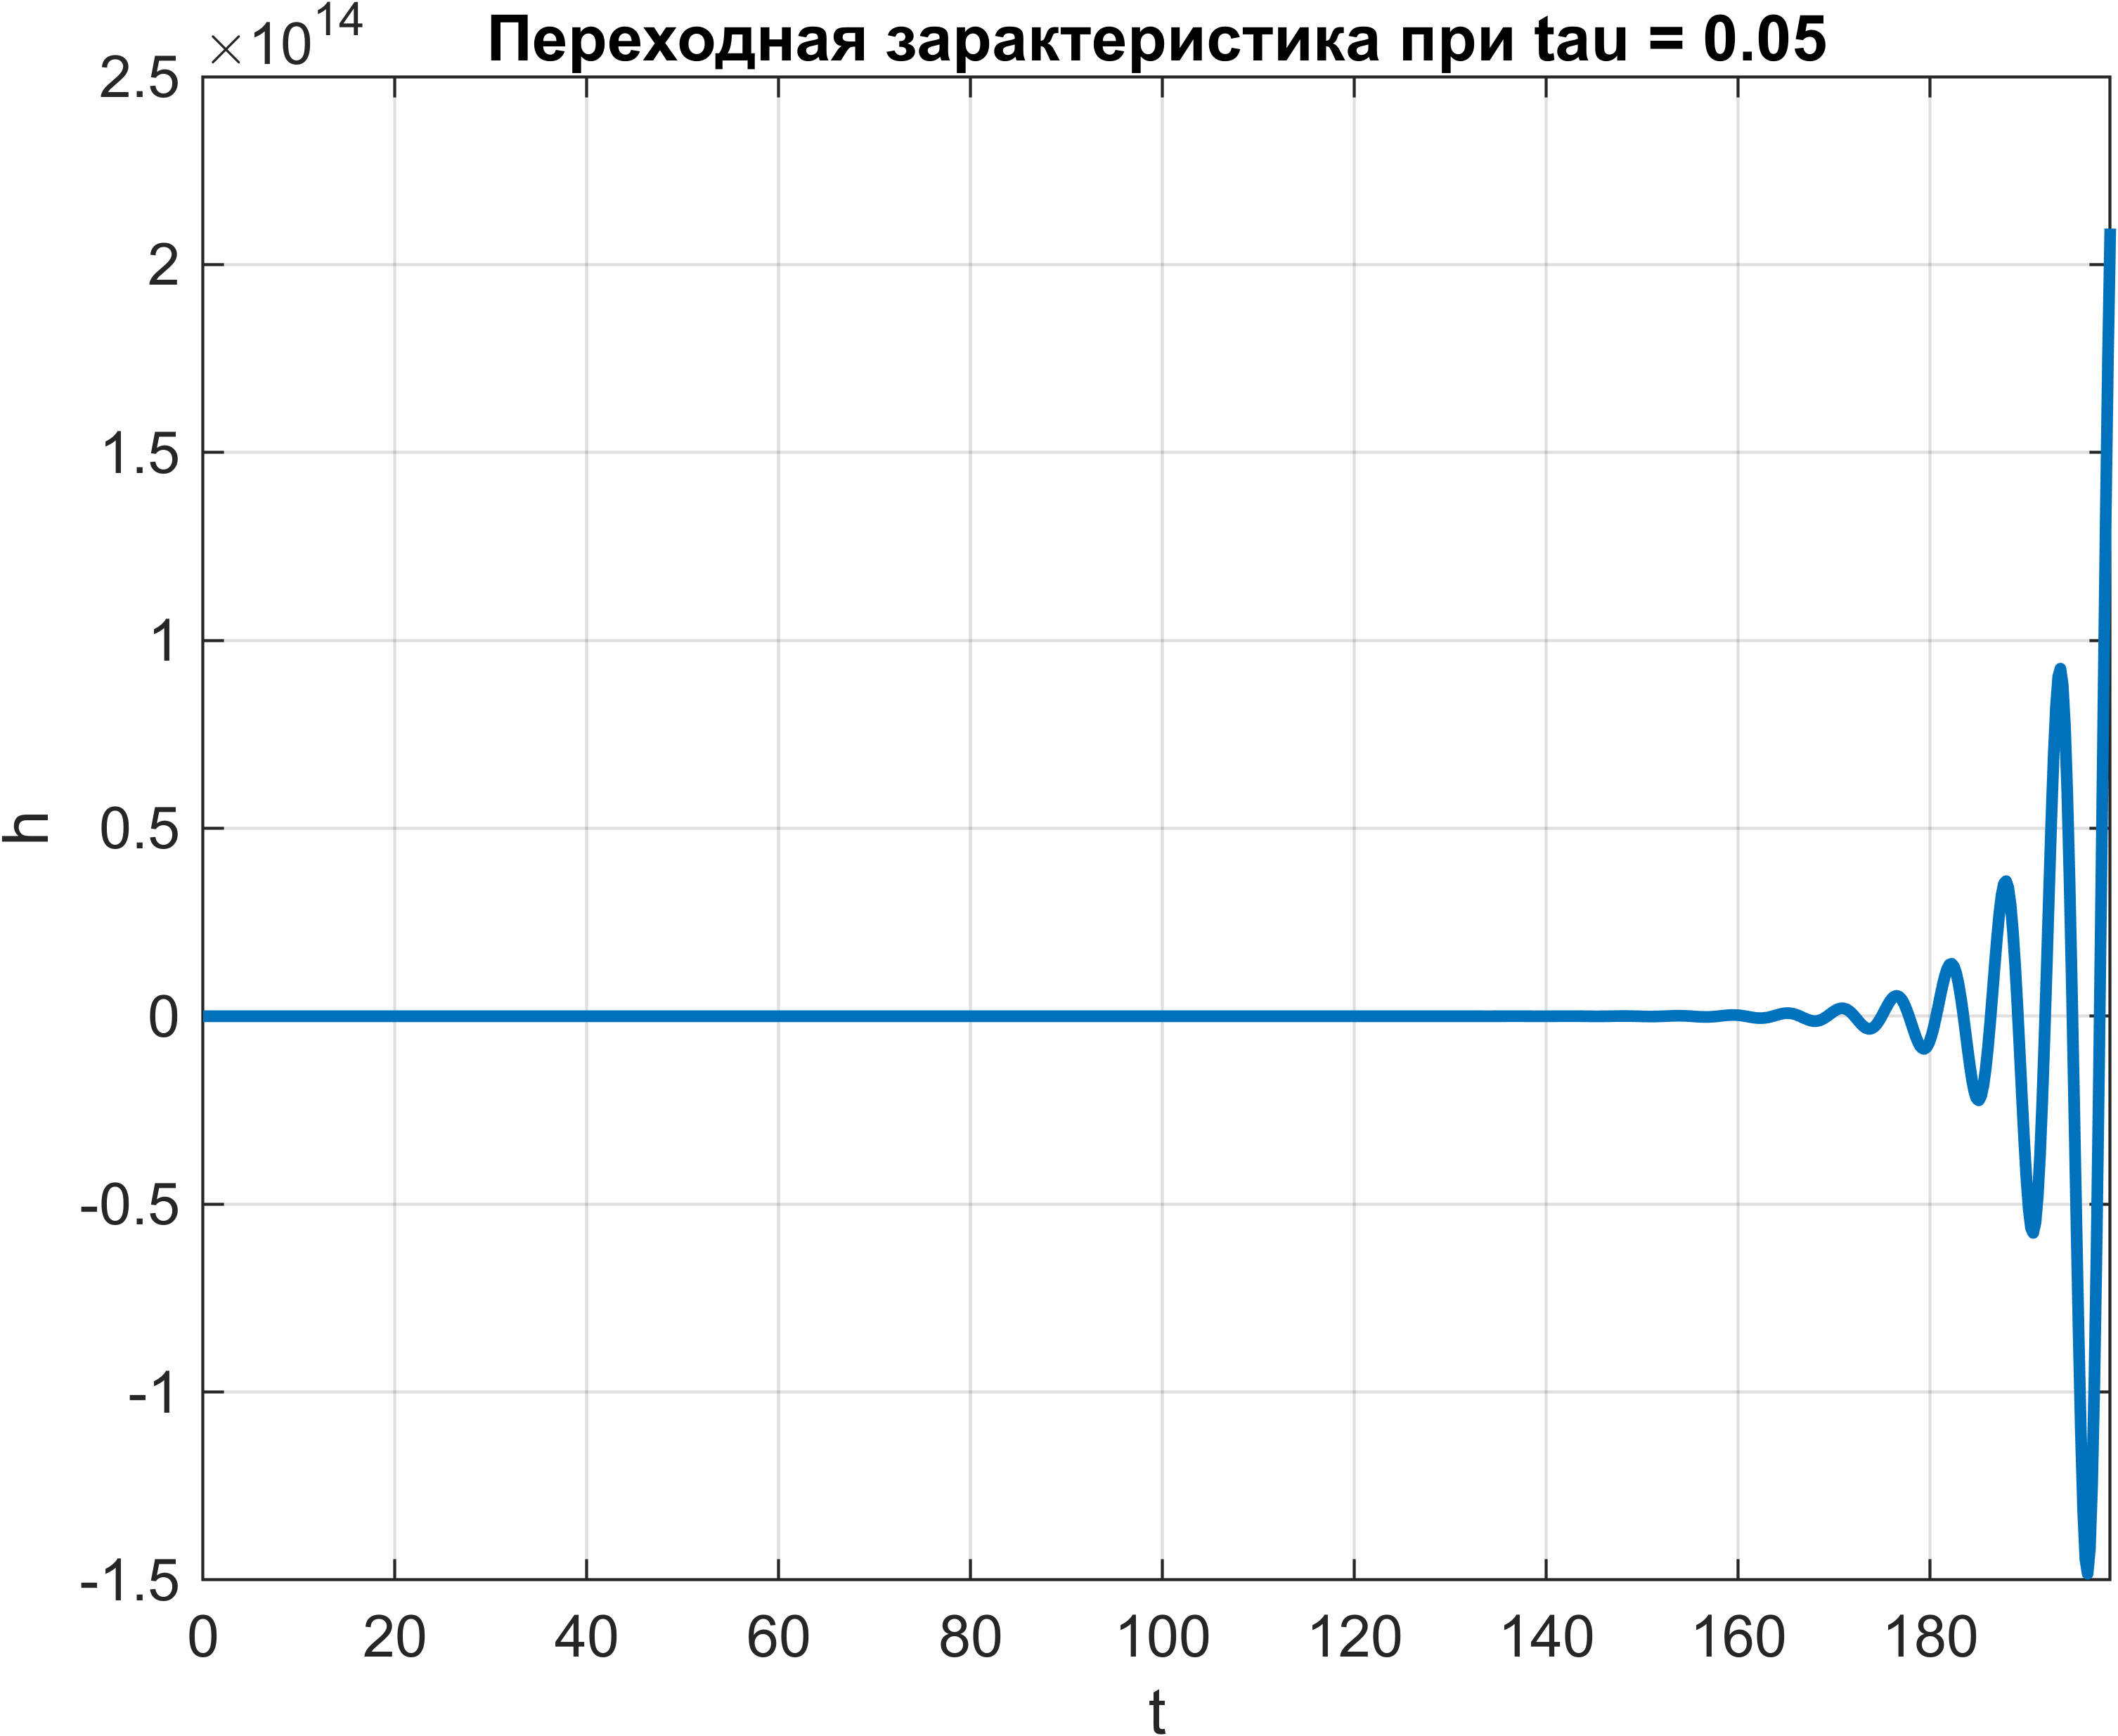
\includegraphics[width=\textwidth, trim={0cm 0cm 0cm 0cm}]{../images/3_2_5_cl.png}
    \end{minipage}
    \hfill
    \begin{minipage}{0.45\textwidth}
        \centering
        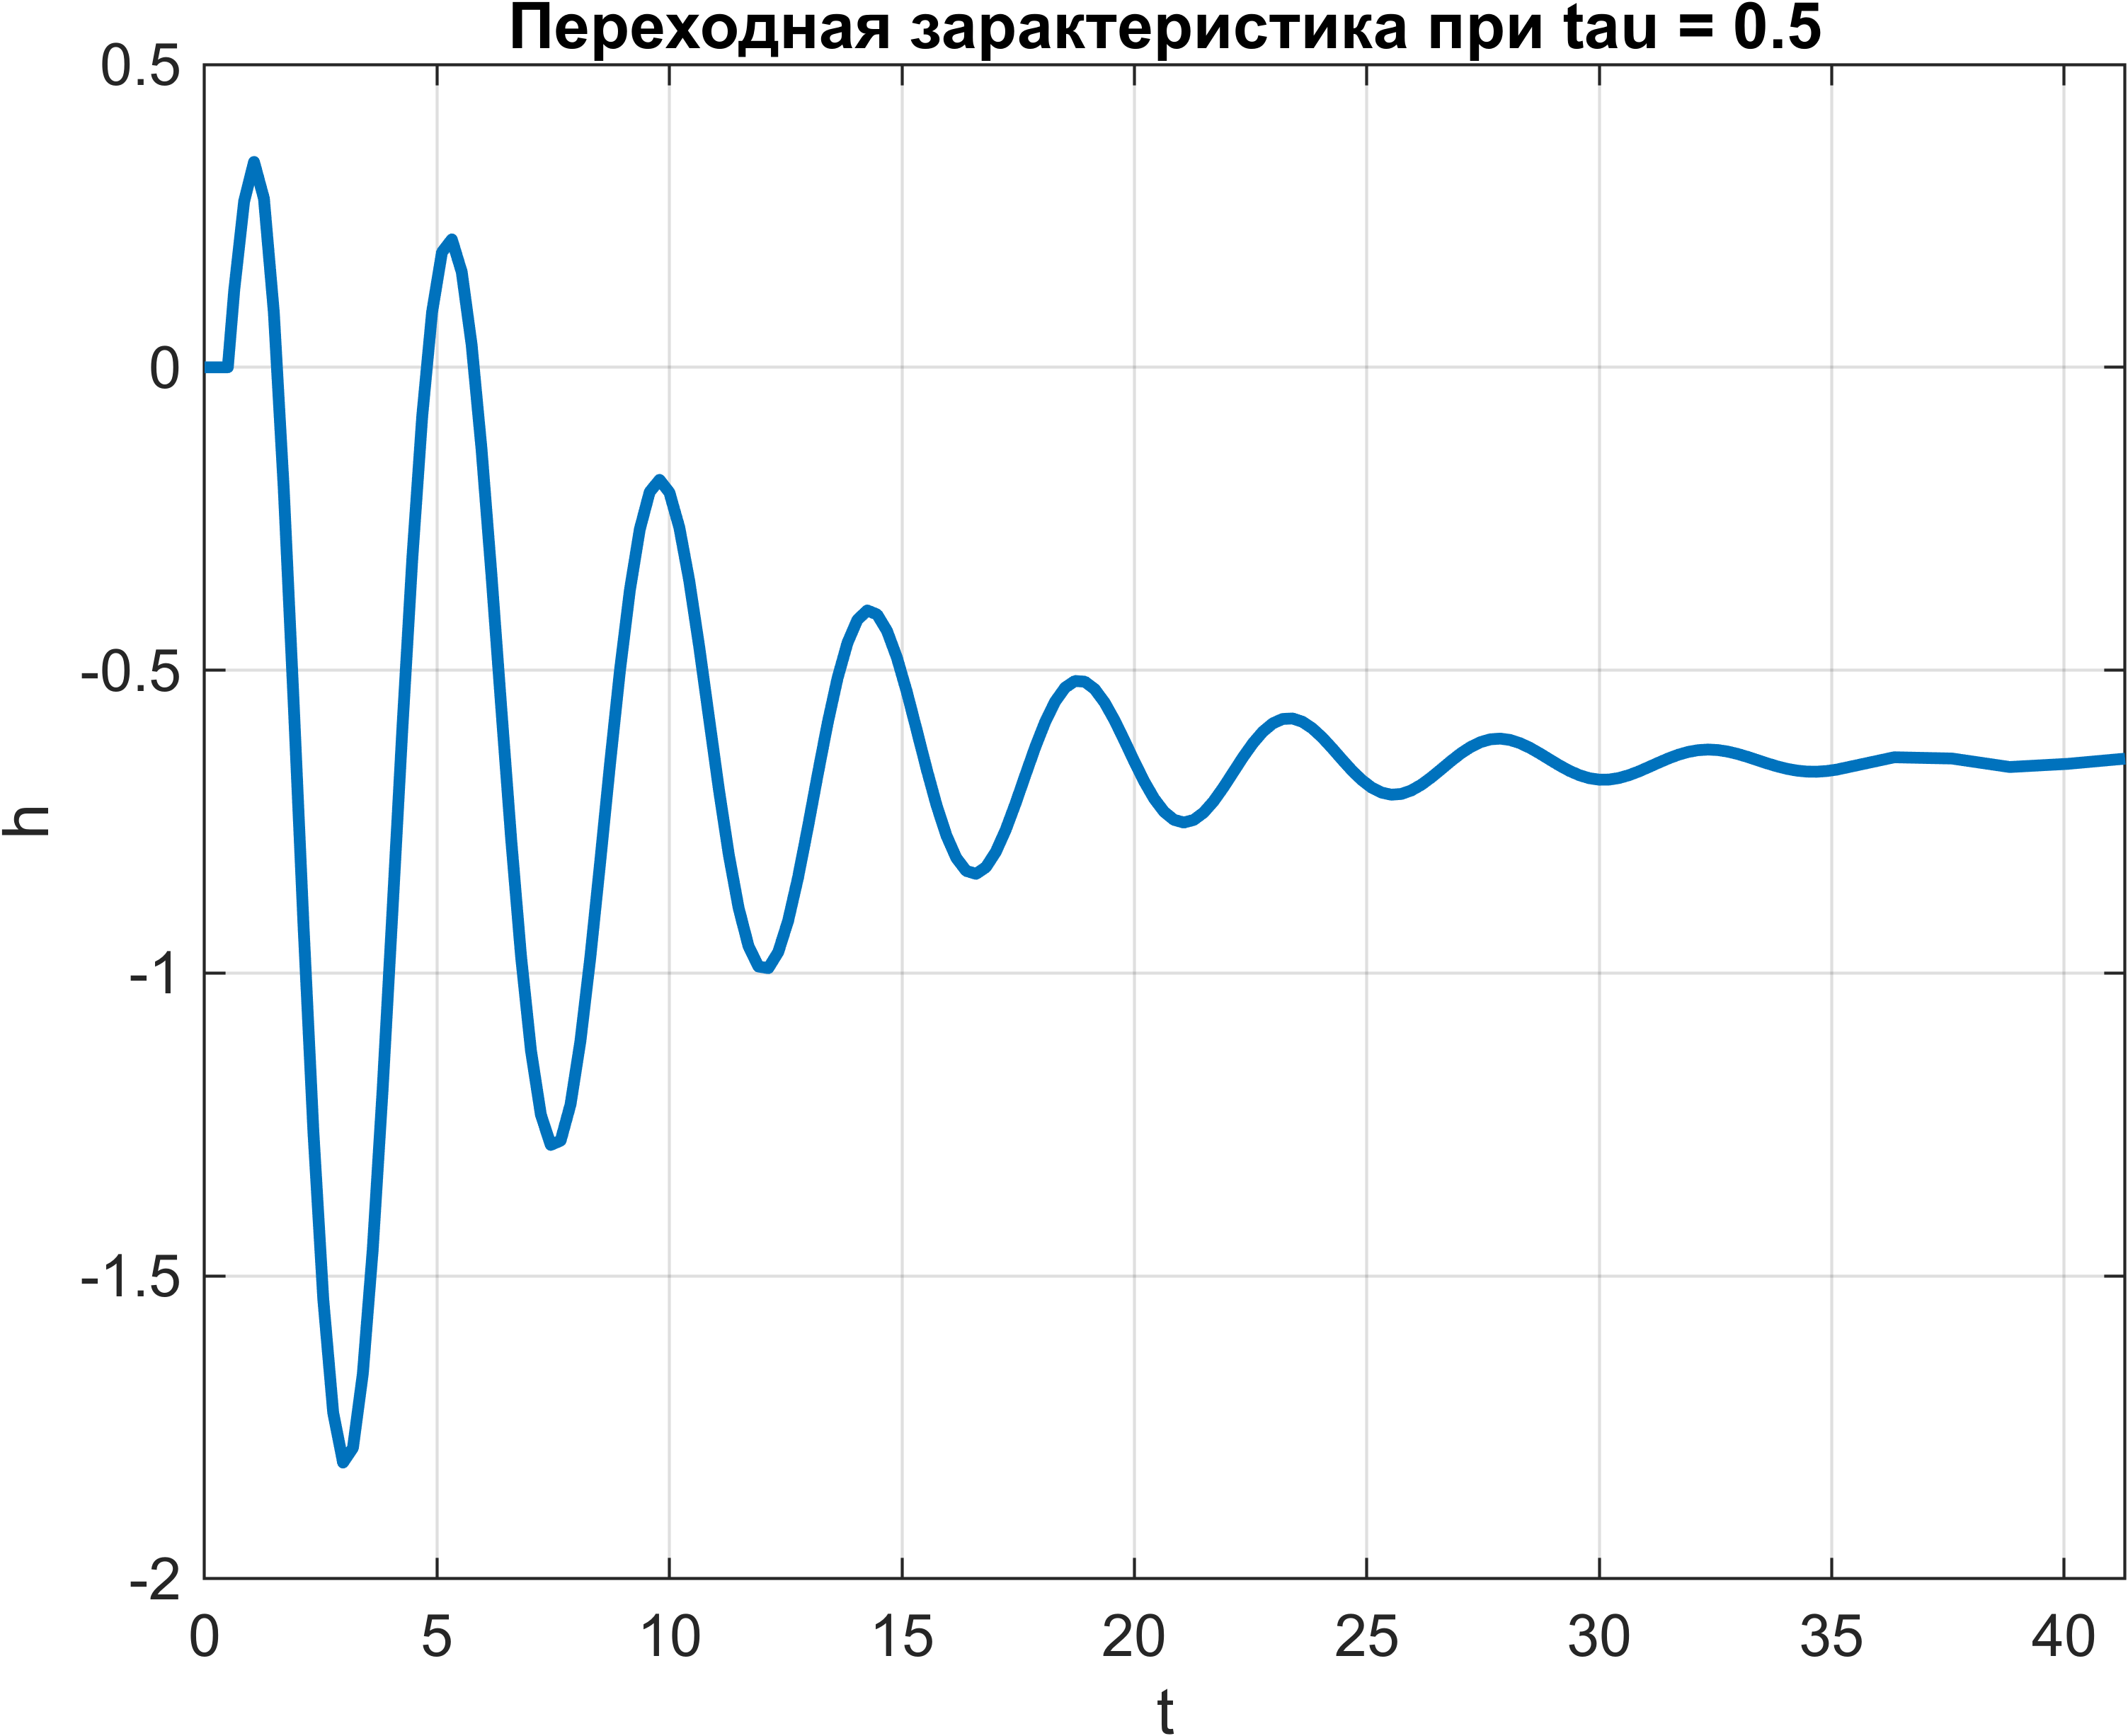
\includegraphics[width=\textwidth, trim={0cm 0cm 0cm 0cm}]{../images/3_2_6_cl.png}
    \end{minipage}
    \vfill
    \begin{minipage}{0.45\textwidth}
        \centering
        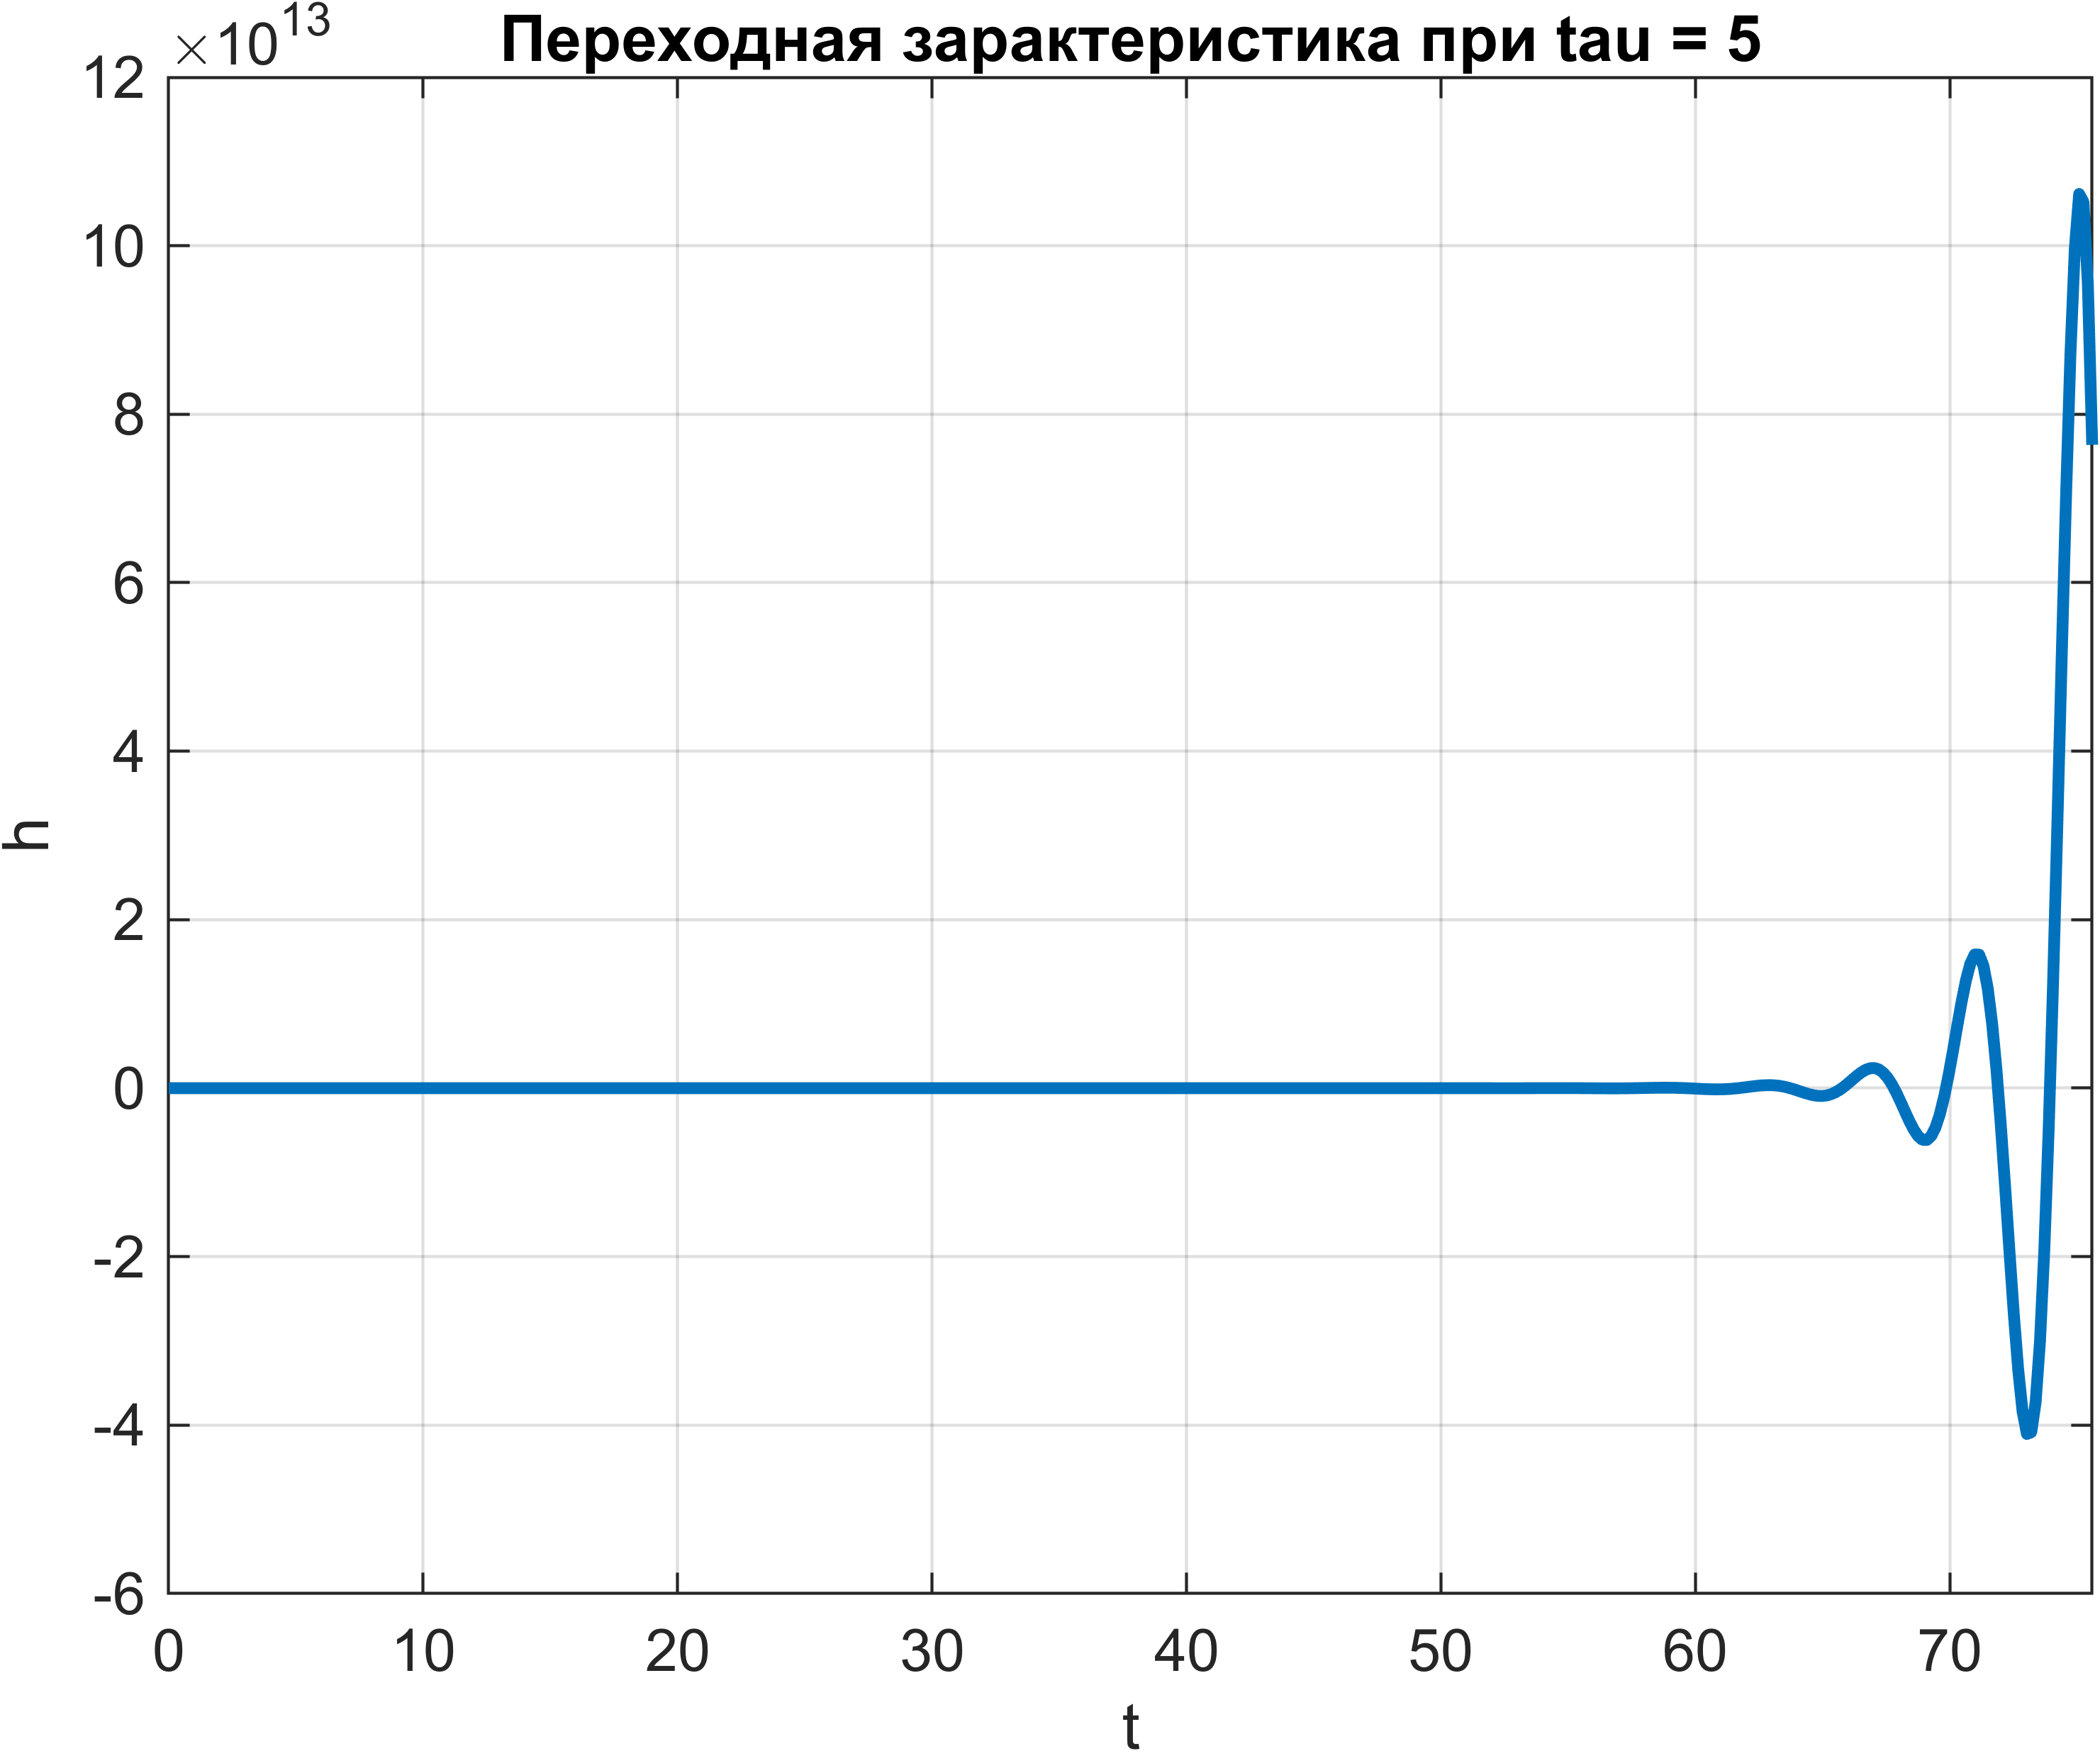
\includegraphics[width=\textwidth, trim={0cm 0cm 0cm 0cm}]{../images/3_2_7_cl.png}
    \end{minipage}
    \hfill
    \begin{minipage}{0.45\textwidth}
        \centering
        % Пустое место для 4-го элемента
    \end{minipage}
    \caption{Переходные характеристики системы для $\tau = 0.05$, $\tau = 1$, $\tau = 5$}
\end{figure}

\endinput